%% ****** Start of file apstemplate.tex ****** %
%%
%% This file is part of the APS files in the REVTeX 4 distribution.
%% Version 4.1r of REVTeX, August 2010
%%
%%
%% Copyright (c) 2001, 2009, 2010 The American Physical Society.
%%
%% See the REVTeX 4 README file for restrictions and more information.
%%
%
% This is a template for producing manuscripts for use with REVTEX 4.0
% Copy this file to another name and then work on that file.
% That way, you always have this original template file to use.
%
% Group addresses by affiliation; use superscriptaddress for long
% author lists, or if there are many overlapping affiliations.
% For Phys. Rev. appearance, change preprint to twocolumn.
% Choose pra, prb, prc, prd, pre, prl, prstab, prstper, or rmp for journal
%  Add 'draft' option to mark overfull boxes with black boxes
%  Add 'showpacs' option to make PACS codes appear
%  Add 'showkeys' option to make keywords appear
\documentclass[aps,pra,reprint,superscriptaddress]{revtex4-1}
%\documentclass[aps,prl,preprint,superscriptaddress]{revtex4-1}
%\documentclass[aps,prl,reprint,groupedaddress]{revtex4-1}

% You should use BibTeX and apsrev.bst for references
% Choosing a journal automatically selects the correct APS
% BibTeX style file (bst file), so only uncomment the line
% below if necessary.
%\bibliographystyle{apsrev4-1}
\usepackage{graphicx}
\usepackage{amssymb, amsmath}
\usepackage{esdiff} % use this package for derivative and partial derivate commands of \diff{}{} and \diffp{}{}
\usepackage{siunitx}
\DeclareSIUnit\cells{cells}

\DeclareMathOperator{\hilbert}{\mathcal{H}} % To define additional named operators
\DeclareMathOperator{\h}{h} % To define additional named operators
\DeclareMathOperator{\unwrap}{unwrap} % To define additional named operators

\begin{document}

% Use the \preprint command to place your local institutional report
% number in the upper righthand corner of the title page in preprint mode.
% Multiple \preprint commands are allowed.
% Use the 'preprintnumbers' class option to override journal defaults
% to display numbers if necessary
%\preprint{}

%Title of paper
\title{High-throughput label-free cell classification using machine learning}

% repeat the \author .. \affiliation  etc. as needed
% \email, \thanks, \homepage, \altaffiliation all apply to the current
% author. Explanatory text should go in the []'s, actual e-mail
% address or url should go in the {}'s for \email and \homepage.
% Please use the appropriate macro foreach each type of information

% \affiliation command applies to all authors since the last
% \affiliation command. The \affiliation command should follow the
% other information
% \affiliation can be followed by \email, \homepage, \thanks as well.
\author{Claire L. Chen}
\email[Email: ]{l.chen@ucla.edu}
%\homepage[]{Your web page}
%\thanks{}
\author{Ata Mahjoubfar}
\affiliation{Department of Electrical Engineering, University of California, Los Angeles, California 90095, USA}
\affiliation{California NanoSystems Institute, Los Angeles, California 90095, USA}
\author{Li-Chia Tai}
\affiliation{California NanoSystems Institute, Los Angeles, California 90095, USA}
\author{Ian Blaby}
\affiliation{Department of Chemistry and Biochemistry, University of California, Los Angeles, California 90095, USA}
\author{Kayvan R. Niazi}
\affiliation{NantWorks, LLC, Culver City, California 90232, USA}
\affiliation{Department of Bioengineering, University of California, Los Angeles, California 90095, USA}
\author{Bahram Jalali}
\affiliation{Department of Electrical Engineering, University of California, Los Angeles, California 90095, USA}
\affiliation{California NanoSystems Institute, Los Angeles, California 90095, USA}
\affiliation{Department of Bioengineering, University of California, Los Angeles, California 90095, USA}
\affiliation{Department of Surgery, David Geffen School of Medicine, University of California, Los Angeles, California 90095, USA}

%Collaboration name if desired (requires use of superscriptaddress
%option in \documentclass). \noaffiliation is required (may also be
%used with the \author command).
%\collaboration can be followed by \email, \homepage, \thanks as well.
%\collaboration{}
%\noaffiliation

\date{\today}

\begin{abstract}
Label-free cell analysis is needed for personalized genomics, cancer diagnostics, and drug development as it avoids adverse effects of staining reagents on cellular viability or cell signaling. However, currently available label-free cell assays mostly rely only on a single feature, namely on cell size or dielectric constant. They also have low throughput limiting the sample size that can be analyzed. Here we report that by combining feature extraction and machine learning to high throughput quantitative phase imaging enabled by the photonic time stretch, cells can be classified with high accuracy. Our system captures quantitative phase images in a flow-through microscope and extracts multiple biophysical features such as morphological parameters, optical loss characteristics, and protein concentration indicators of individual cells. These biophysical measurements form a hyperdimensional feature space in which supervised learning is performed for cell classification. As a validation of the enhanced classification sensitivity and specificity of our method, we show binary classification of OT-II white blood T-cells against SW-480 colon cancer cells. Additionally, we show classification of lipid accumulating algal strains for biofuel production. This system opens up a new path to data-driven genotype trained phenotype diagnosis and better understanding of the heterogeneous phenotypic expressions in cells.
\end{abstract}

% insert suggested PACS numbers in braces on next line
%\pacs{}
% insert suggested keywords - APS authors don't need to do this
\keywords{Label-free cell analysis, Quantitative phase imaging, Time stretch, Dispersive Fourier transform.}

%\maketitle must follow title, authors, abstract, \pacs, and \keywords
\maketitle

% body of paper here - Use proper section commands
% References should be done using the \cite, \ref, and \label commands

Conventional flow cytometry is a powerful tool for large-scale cell analysis due to its ability to measure anisotropic elastic light scattering of millions of individual cells as well as emission of fluorescent labels conjugated to cells \cite{shapiro2005practical,watson2004introduction}. However each cell is represented with single values per detection channels (forward scatter, side scatter, and emission bands), requiring labeling with specific biomarkers for acceptable classification accuracy \cite{shapiro2005practical,perfetto2004seventeen}. Imaging flow cytometry \cite{basiji2007cellular,basiji2001imaging} on the other hand captures images of cells revealing significantly more information about the cells. For example, it can distinguish clusters and debris that would otherwise result in false positive identification in a conventional flow cytometer based on light scattering \cite{carpenter2006cellprofiler}.

In addition to classification accuracy, another critical specification of a flow cytometer is its throughput. Indeed high throughput, typically 100,000 cells per second, is needed to screen a large enough cell population to find rare abnormal cells that are indicative of early stage disease. However there is a fundamental trade-off between throughput and accuracy in any measurement system \cite{razavi1995principles,mahjoubfar2013optically}. Additionally, imaging flow cytometers face a throughput limit imposed by the speed of the CCD or the CMOS cameras, a number that is approximately 2000 cells/s for present systems \cite{goda2012high}. Higher flow rate lead to blurred cell images due to the finite camera shutter speed. Many applications of flow analyzers such as cancer diagnostics, drug discovery, biofuel development, and emulsion characterization require classification of large sample sizes with a high-degree of statistical accuracy \cite{zanella2010high}. This has fueled research into alternative optical diagnostics techniques for characterization of cells and particles in flow.

Recently, our group has developed a label-free imaging flow-cytometry technique based coherent optical implementation of the photonic time stretch concept \cite{mahjoubfar2013label}. The instrument overcomes the trade-off between sensitivity and speed by using Amplified Time-stretch Dispersive Fourier Transform (ADFT) \cite{goda2013dispersive, solli2009optical, goda2009theory}. In time stretched imaging \cite{goda2009serial}, the object's spatial information is encoded in a spectrum of laser pulses within a pulse duration of sub-nanoseconds (Fig.~\ref{fig:Setup}). Each pulse representing one frame of the camera is then stretched in time so that it can be digitized in real-time by an electronic analog-to-digital converter. The ultra-fast pulse illumination freezes the motion of high-speed cells or particles in flow to achieve blur-free imaging. Detection sensitivity is challenged by the low number of photons collected during the ultra-short shutter time (optical pulse width) and the drop in the peak optical power resulting from the time stretch. This issue is solved in time stretch imaging by implementing a low noise-figure Raman amplifier within the dispersive device that performs time stretching \cite{goda2009serial,mahjoubfar2013label,mahjoubfar2013optically}. In the coherent version of the instrument utilized here, the time stretch imaging is combined with spectral interferometry to measure quantitative phase images in real-time and at high throughput \cite{mahjoubfar2014label}. Integrated with a microfluidic channel, coherent time stretch imaging system in this work captures 36 million quantitative phase and intensity images of individual cells every second in flow rates as high as 10 meters per second with a throughput up to 100,000 cells per second as a high-speed imaging flow cytometer.

\begin{figure*}
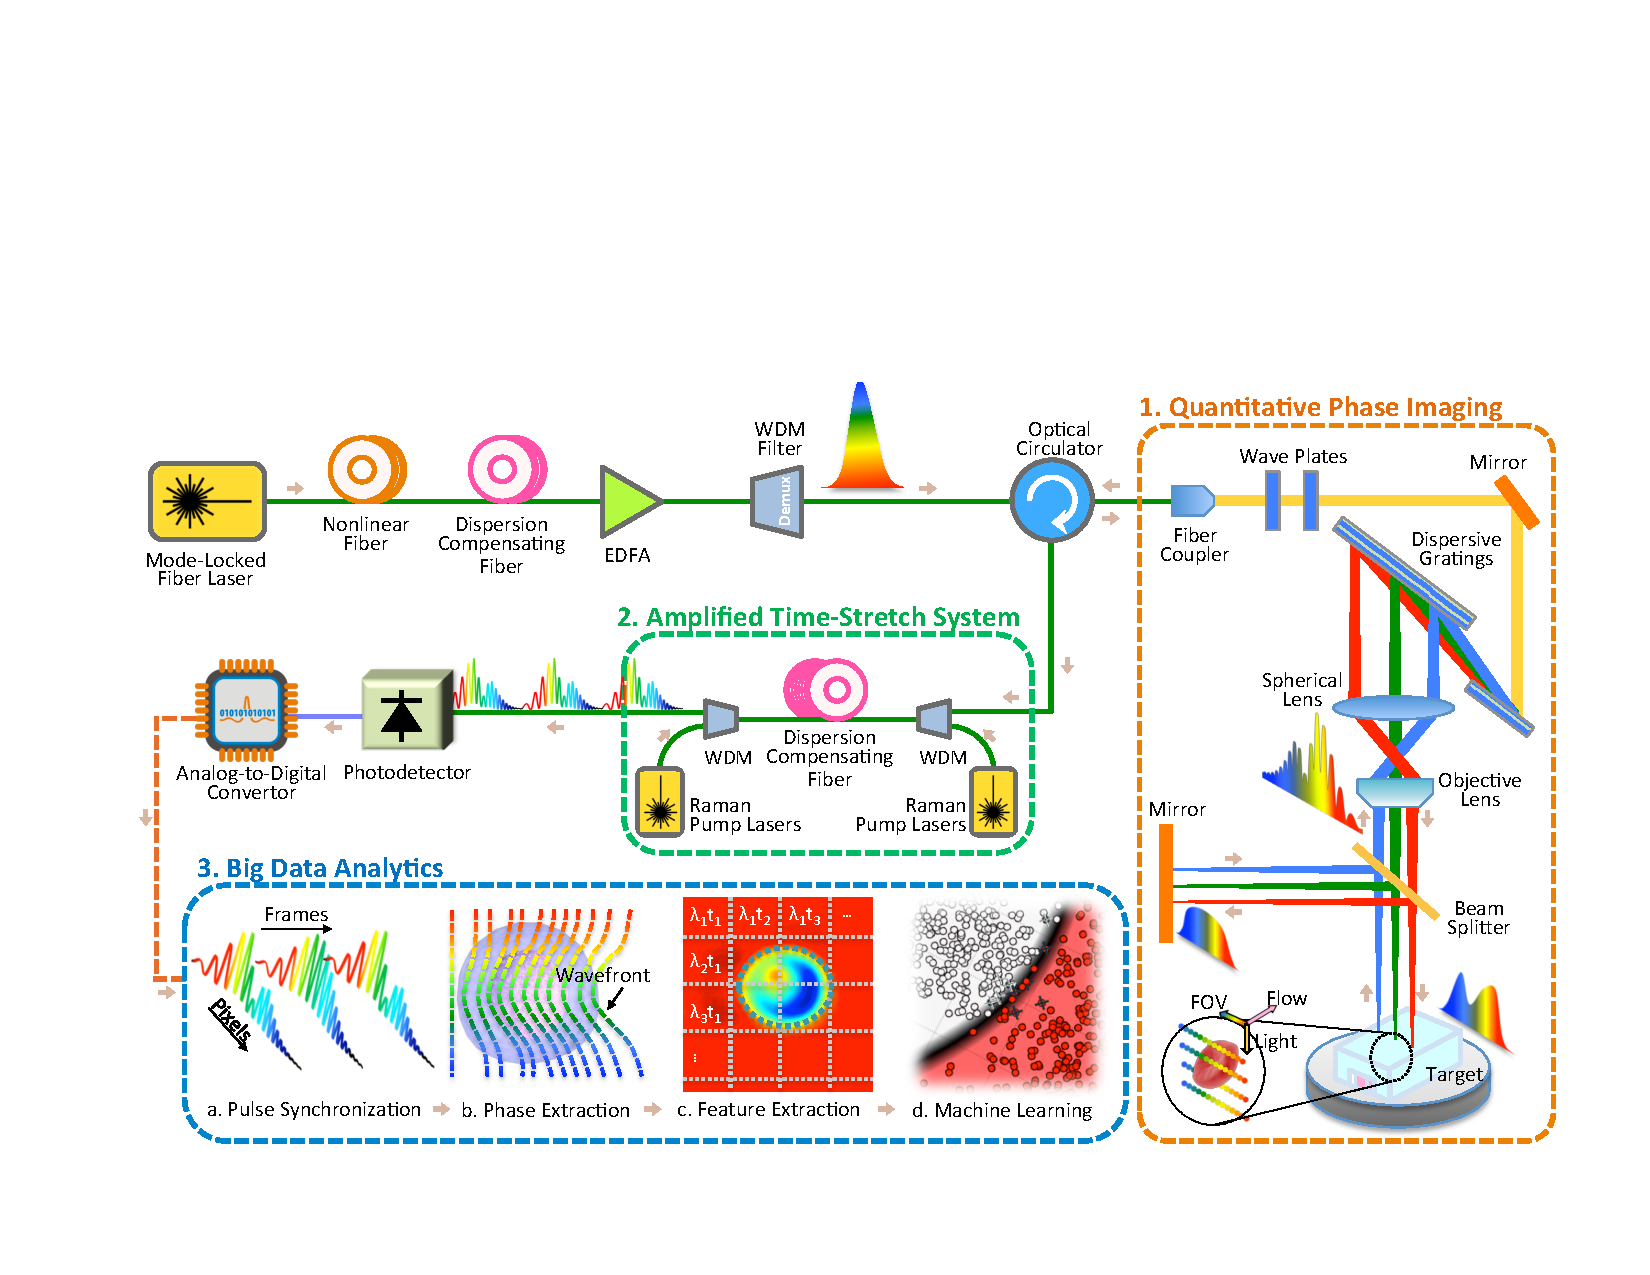
\includegraphics[scale=0.70]{FigureSetup.pdf}
\caption{\label{fig:Setup} Time stretch quantitative phase imaging (TS-QPI) and analytics system; A mode-locked laser followed by a nonlinear fiber, an erbium doped fiber amplifier (EDFA), and a wavelength-division multiplexing (WDM) filter generate and shape a train of broadband optical pulses. Box 1: The pulse train is spatially dispersed into a train of rainbow flashes illuminating the target as line scans. The spatial features of the target are encoded into the spectrum of the broadband optical pulses each representing a one-dimensional frame. The ultra-short optical pulse illumination freezes the motion of cells during high speed flow to achieve blur-free imaging with a throughput of 100,000 cells/s (limited by the flow channel). The phase shift at each location within the field of view is embedded into the spectral interference patterns using by a Michelson interferometer. Box 2: The interferogram pulses were then stretched in time so that spatial information could be mapped into time through time-stretch dispersive Fourier transform (TS-DFT), and then captured by a single pixel photodetector and an analog-to-digital converter (ADC). The loss of sensitivity at high shutter speed is compensated by stimulated Raman amplification during time stretch. Box 3: (a) Pulse synchronization; the time-domain signal carrying serially captured rainbow pulses is transformed into a series of one-dimensional spatial maps, which are used for forming line images. (b) The biomass density of a cell leads to a spatially varying optical phase shift. When a rainbow flash passes through the cells, the changes in refractive index at difference locations will cause phase walk-off at interrogation wavelengths. Hilbert transformation and phase unwrapping are used to generate the spatial information of phase shift. (c) Decoding the phase shift in each pulse at each wavelength and remapping it into a pixel reveals the protein concentration distribution within cells. The optical loss induced by the cells, embedded in the pulse intensity variations, is obtained from the amplitude of the slowly varying envelope of the spectral interferograms. Thus, quantitative optical phase shift and intensity loss images are captured simultaneously. Both images are calibrated based on the regions where the cells are absent. Cell features describing morphology, granularity, biomass, etc are extracted from the images. (d) These biophysical features are used in a machine learning algorithm for high-accuracy label-free classification of the cells.}
\end{figure*}

On another note, surface markers used to label cells, such as EpCAM, are an indispensable tool for cell classification. However, they are unavailable in some applications; for example, melanoma or pancreatic circulating tumor cells as well as some cancer stem cells are EpCAM-negative and will escape EpCAM-based detection platforms \cite{kling2012beyond}. Furthermore, large-population cell sorting opens the doors to downstream operations where the negative impacts of labels on cellular behavior and viability are often unacceptable \cite{boddington2011labeling}. Cell labels may cause activating/inhibitory signal transduction, altering the behavior of the desired cellular subtypes, potentially leading to errors in downstream analysis, such as DNA sequencing and subpopulation regrowth. In this way, quantitative phase imaging (QPI) methods \cite{ikeda2005hilbert,popescu2011quantitative,pham2013real} that categorize unlabeled living cells with high accuracy are needed. Coherent time stretch imaging is a method that combines QPI with high throughput imaging for non-invasive screening of large number of cells in flow.

In this work, image mining and machine learning techniques are applied, for the first time, to label-free time stretch QPI to measure biophysical parameters corresponding to protein concentration, optical loss, and morphological features on single cells with an ultrahigh flow rate and in a label-free fashion. As protein concentration and morphology in mammalian cells differ widely \cite{feinerman2008variability, sigal2006variability, friebel1999optical, vona2000isolation} and their variations reflect important information of genotypes and physiological stimuli \cite{spencer2009non}. These multiplexed biophysical parameters then lead to information-rich hyper-dimensional scatter plots for label-free cell classification with high statistical precision. To demonstrate sensitivity, specificity, and accuracy of multi-parameter label-free flow cytometry using our technique, we classified (1) OT-II hybridoma T-lymphocytes and SW-480 colon cancer epithelial cells, and (2) Chlamydomonas reinhardtii algal cells (herein referred to as Chlamydomonas) based on their lipid content, which is related to their use in biofuel production. Our preliminary results show that compared to classification by individual biophysical parameters, our label-free hyperdimensional technique improves the detection accuracy from 78.1\% to 95.5\%, or in other words, reduces the classification inaccuracy by about five times. 

\section{Results}
\subsection{Time Stretch Quantitative Phase Imaging}

The application of time stretch quantitative phase imaging (TS-QPI) to imaging flow cytometry has been recently demonstrated in our group \cite{mahjoubfar2013label}. Broadband optical pulses from a mode-locked laser were firstly conditioned in fiber optics and then spatially dispersed in free-space optics with a pair of reflection diffraction gratings creating 1-D ``rainbow flashes'' (Fig.~\ref{fig:Setup}). Each of rainbow flashes was composed of all the wavelength components distributed laterally over the field of view. These flashes illuminated the target as in traditional photography, but in addition, rainbow flashes targeted different spatial points with distinct colors of light, resulting in space-to-spectrum encoding. Rainbow pulses were then split into the two arms of a Michelson interferometer. Different wavelength components of the rainbow flash traveled parallel to each other but individually focused on the mirror in the reference arm or on the reflective substrate of a microfluidic device in the sample arm. In the sample arm, the cells in the microfluidic channel were hydrodynamically focused \cite{knight1998hydrodynamic,lee2006hydrodynamic} into the rainbow's field of view and flowed perpendicular to the rainbow flash. Reflected pulses from the microfluidic device and the reference arm were recombined and coupled back into the fiber, optically amplified and linearly chirped through Raman-amplified TS-DFT system. An ultrafast single-pixel photodetector  transformed instantaneous optical power into an electrical signal and subsequently, an analog-to-digital convertor (ADC) samples and quantizes the signal. Acquired data are passed down to processing stages for big data analytics. The interference between time-shifted linearly chirped pulses create a beat (fringe) frequency, which can be adjusted via the interferometer arm length mismatch.

High speed phase contrast imaging was achieved with high sensitivity using an amplified time-stretch system that creates a low-noise distributed Raman amplifier within dispersive fiber with a net optical image gain of approximately 15 dB. The photodetected time-stretched pulses, each representing one line-scan, are converted to analytic signals using Hilbert transformation \cite{king2009hilbert} and the phase component is extracted. Since the phase varies over a wide range (much larger than $2 \pi$ radians), an unwrapping algorithm is used to obtain the continuous phase profile. The phase profile contains an increasing term with time, corresponding to the fringe (beat) frequency and the phase shift induced by the cell. By eliminating the background phase component, the cell-induced phase shift is extracted, from which a 2D phase image is constructed (Fig.~\ref{fig:2DImage}).

\begin{figure*}
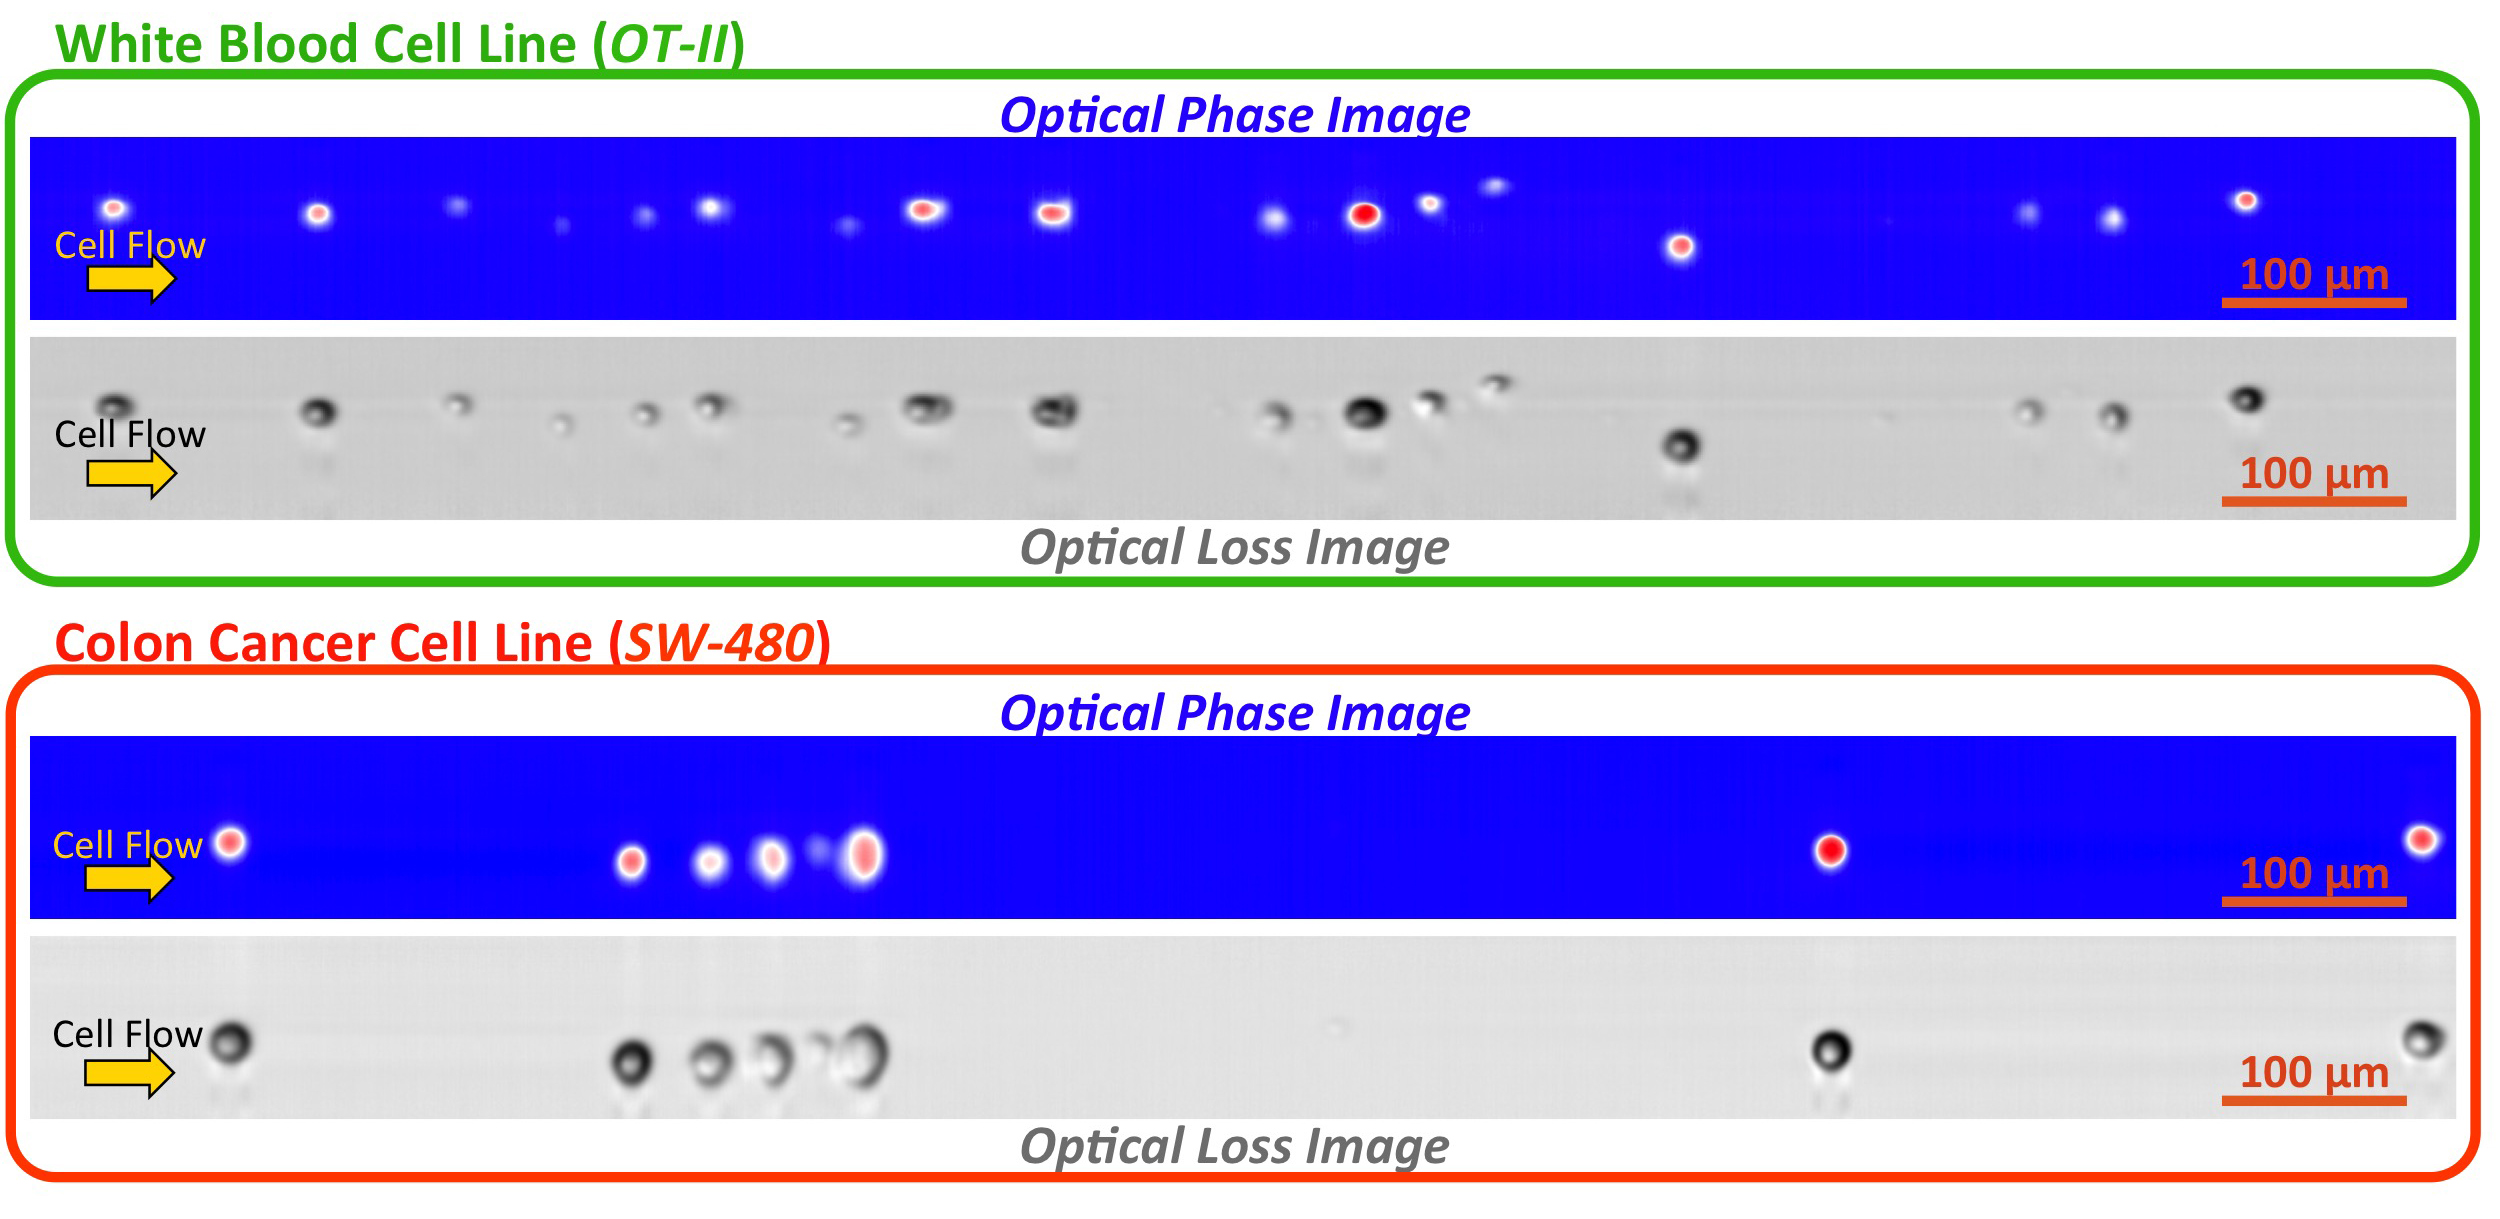
\includegraphics[scale=0.5]{Figure2DImage.jpg}
\caption{\label{fig:2DImage} Quantitative phase and optical loss images of OT-II (blue) and SW-480 (green box) cells. The optical loss images of the cells are affected by the attenuation of multiplexed wavelength components passing through the cells. The attenuation itself is governed by the absorption of the light in cells as well as the scattering from the surface of the cells and from the internal cell organelles. The optical loss image is derived from the low frequency features of the pulse interferograms. The optical phase image is extracted from the analytic form of the high frequency features of the pulse interferograms using Hilbert Transformation, followed by a phase unwrapping algorithm. Details of these derivations can be found in Section \ref{scn:Methods}.}
\end{figure*}

The time stretched temporal waveforms corresponding to each line scan consists of two features. One is a fast oscillating fringe (carrier), caused by the interference of the linearly chirped pulses arriving from the reference and signal arms in the Michelson interferometer. Acting as a radio-frequency (RF) carrier whose frequency is set by the user adjusted arm length mismatch, the fringe frequency is modulated when the optical path length in the sample arm is changed by the arrival of a cell. This frequency shift and the accompanying phase change are used to measure the optical path length of the cell. The second feature in the waveform is a lower frequency envelope corresponding to temporal shape of the optical pulse. The amplitude of this envelope provides information about optical loss caused by surface roughness and inner organelle complexity (Fig.~\ref{fig:2DImage}). 

One of the challenges in imaging flow cytometry is the uncertainty in the position of the cell along the optical axis. Since the optical path length is a quantity that is integrated over the entire depth along the axis, maps of optical path lengths are mostly insensitive to axial position of the cells. The refractive index used as a measure of protein density is obtained by dividing the measured optical path length by the cell thickness. Since cells in suspension relax to a spherical shape (due to surface tension) \cite{revel1974adhesion,whur1977substrate}, an independent measure of cell diameter can be obtained from its lateral dimension. Finally, the optical loss of each cell is obtained from the amplitude of the slowly varying envelope as discussed previously.

\subsection{Feature Extraction}

Instead of producing a single value from each cell image, we make quantitative image analysis and measure variety of features for large population of cells. The 2D image obtained from sequential linescans provides spatial information about cell \cite{mahjoubfar2013optically, driscoll2012automated}. Owing to the high throughput of the time-stretch quantitative phase imager (TS-QPI), multiple parameters of individual cells can be extracted for a large cell population. The measured cell information not only includes morphology, such as diameter, area, shape, aspect ratio, uniformity, etc., but also biophysical features such as protein concentration, absorption, and scattering.

It is well known that cells from the same line or tissue exhibit variations in size, structure, and protein expression levels, even when they are genetically identical \cite{kaern2005stochasticity, maheshri2007living}. These intrinsic variations have important role in analyzing important extrinsic variations caused by drug treatment \cite{spencer2009non}, cell cycles, labeling, and transcription rate \cite{johnston2012mitochondrial}. The large data set captured by the phase contrast time stretch imaging flow cytometer provides statistically relevant biophysical information that is useful in drug development.

We have developed a feature extraction tool that performs segmentation, object detection and feature measurement. The algorithm operates on optical phase and loss images simultaneously. The analysis also includes clump identification noise suppression, and smoothing applied before cell identification. In our feature extraction, the morphology of each single cell is described by area, diameter along interrogation rainbow, major axis, minor axis, orientation, median radius, circularity, perimeter, and number of surrounding clumped cells. The change in optical pulse intensity caused by cell absorption and scattering is extracted from the pixel intensities in the optical loss image. Cell protein concentration is extracted from the pixel intensities in the phase image \cite{barer1953refractometry}. Overall, 16 major features are shown here for each cell. The relative efficacy of these parameters in cell classification are quantified below.

Among different features, size measurement is particularly important as it is used as a fundamental parameter by itself in many technologies \cite{adams2008highly, nagrath2007isolation, vona2000isolation, gossett2010label}, but also used to extract the refractive index (and hence protein level) from measured optical path length here. Size measurement is performed along both the lateral (rainbow flashes) and flow directions. The measurement along the rainbow direction is used for protein concentration estimation since it helps to eliminate measurement inaccuracies caused by fluctuations of flow speed. We also measure the aspect ratio, perimeter, and median radius as well as a host of other parameters listed in Table~\ref{tbl:Features}. To calibrate the system, we used \SI{5}{\micro\meter} polystyrene beads (from Polysciences, Inc.) with a narrow and known NIST traceable size distribution.

\begin{table*}
\caption{\label{tbl:Features} List of extracted features}
\begin{tabular}{|p{0.13\textwidth}|p{0.6\textwidth}|p{0.11\textwidth}|}
\hline
Feature Name	 &Description	 &Category\\ \hline
Diameter-RB	 &Diameter along the interrogation rainbow. It is insensitive to flow rate fluctuation. For higher accuracy, it is calibrated by the spatial nonuniform distribution of rainbow wavelengths. 	 &Morphology\\ \hline
Diameter-FL	 &Diameter along the flow direction. It is sensitive to flow rate fluctuation, but can be a candidate parameter for monitoring flow speed and channel condition.	 &Morphology\\ \hline
Tight Area	 &Total number of pixels in the segmented region in the phase image	 &Morphology\\ \hline
Perimeter	 &Total number of pixels around the boundary of each segmented region	 &Morphology\\ \hline
Circularity	 &$4\pi \text{Area} / \text{Perimeter}^2$  &Morphology\\ \hline
Major Axis 	 &Considering the cell as elliptical in lateral imaging plane, the length of the major axis of the ellipse with a normalized second central moment same as the cell.	 &Morphology\\ \hline
Orientation	 &Angle between the flow direction and the major axis of the cell elliptical shape	 &Morphology\\ \hline
Loose Area	 &Total number of pixels in the expanded segmented region for measurement of the pixel intensities	 &Morphology\\ \hline
Median Radius	 &The median distance of any pixel in the object to the closest pixel outside of the object.	 &Morphology\\ \hline
OPD-1	 &Integrated optical path length difference within the entire segmented area (cell), calibrated by the power distribution within different wavelength components of the incident laser pulses.	 &Optical Phase\\ \hline
OPD-2	 &Integrated optical path length difference within the entire segmented area (cell). In addition to the calibration of OPD-1, it is calibrated by the pulse-to-pulse fluctuations within a \SI{1}{\micro\second} detection window.	 &Optical Phase\\ \hline
Refractive index	 &The mean refractive index difference between the object and the surrounding liquid (buffer solution), which is calculated based on OPD-2 and size measurement (see detail in Section \ref{scn:Methods}). Refractive index difference for cells is proportional to their protein concentration.	 &Optical Phase\\ \hline
Absorption-1	 &Mean absorption coefficient within the entire segmented area (cell). It is calibrated by the power distribution within different wavelength components of the incident laser pulses and by the pulse-to-pulse fluctuations within a \SI{1}{\micro\second} detection window. This parameter corresponds to an absorption-dominant model for the cell.	 &Optical Loss\\ \hline
Absorption-2	 &Mean absolute absorption coefficient within the entire segmented area (cell). It is calibrated by the power distribution within different wavelength components of the incident laser pulses and by the pulse-to-pulse fluctuations within a \SI{1}{\micro\second} detection window. This parameter corresponds to an absorption-dominant model for the cell.	 &Optical Loss\\ \hline
Scattering-1	 &Mean optical loss within the entire segmented area (cell). It is calibrated by the power distribution within different wavelength components of the incident laser pulses and by the pulse-to-pulse fluctuations within a \SI{1}{\micro\second} detection window. This parameter corresponds to a scattering-dominant model for the cell.	 &Optical Loss\\ \hline
Scattering-2	 &Mean absolute optical loss within the entire segmented area (cell). It is calibrated by the power distribution within different wavelength components of the incident laser pulses and by the pulse-to-pulse fluctuations within a \SI{1}{\micro\second} detection window. This parameter corresponds to a scattering-dominant model for the cell.	 &Optical Loss\\
\hline
\end{tabular}
\end{table*}
% \begin{table}%[H] add [H] placement to break table across pages
% \caption{\label{}}
% \begin{ruledtabular}
% \begin{tabular}{}
% Lines of table here ending with \\
% \end{tabular}
% \end{ruledtabular}
% \end{table}

We used hyper-dimensional scatter plots as a tool for high content cell analysis. To demonstrate application in circulating cancer cell (CTC) detection, we used a white blood cell line (OT-II hybridoma T cell) and a cancer cell line (SW-480 epithelial colon cancer). Fig.~\ref{fig:OTSWScatter} shows the 3D scatter plot based on size, protein concentration, and attenuation of a large number of OT-II (black dots) and SW-480 (red dots) cells. The attenuation is a parameter describing the optical intensity loss caused by cell absorption (Absorption-1 feature in Table \ref{tbl:Features}). The 2D projections on the three orthogonal planes are also shown. It is clear that certain pairs of features are better able to differentiate the two populations.

\begin{figure*}
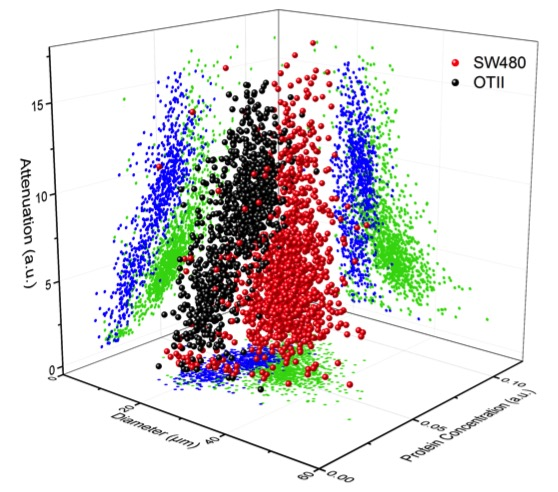
\includegraphics[scale=0.6]{FigureOTSWScatter.jpg}
\caption{\label{fig:OTSWScatter} Three-dimensional scatter plot based on size, protein concentration, and attenuation of OT-II and SW-480 cells measured by TS-QPI; The green and blue dots are two-dimensional (2-D) projections of cell data points on the planes containing only two of the biophysical parameters. The cell protein concentration corresponds to the mean refractive index difference of the cell (Refractive index feature in Table \ref{tbl:Features}). The attenuation is a parameter describing the optical intensity loss caused by cell absorption (Absorption-1 feature in Table \ref{tbl:Features}). Comparison of 2-D scatter plots reveals that additional biophysical parameters (in this case protein concentration) serve to classify the cell types more accurately.}
\end{figure*}

As previously mentioned, a total of 16 features are extracted from optical phase and loss images of each cell. Parameters that are highly correlated do not provide unique information. Pairwise correlation matrix among 16 parameters extracted from the images is shown as a heat map in Fig.~\ref{fig:Correlation}. Diagonal elements of the matrix are correlation of each parameter with itself, i.e. the autocorrelation. The set of parameters with the red color are highly correlated. The subset in the lower left shows high correlation because they all measure morphological features. Also, the subset in the upper right are correlated as they all measure optical loss. This suggests that the dataset can be adequately represented by a smaller set that excludes highly correlated parameters.

\begin{figure*}
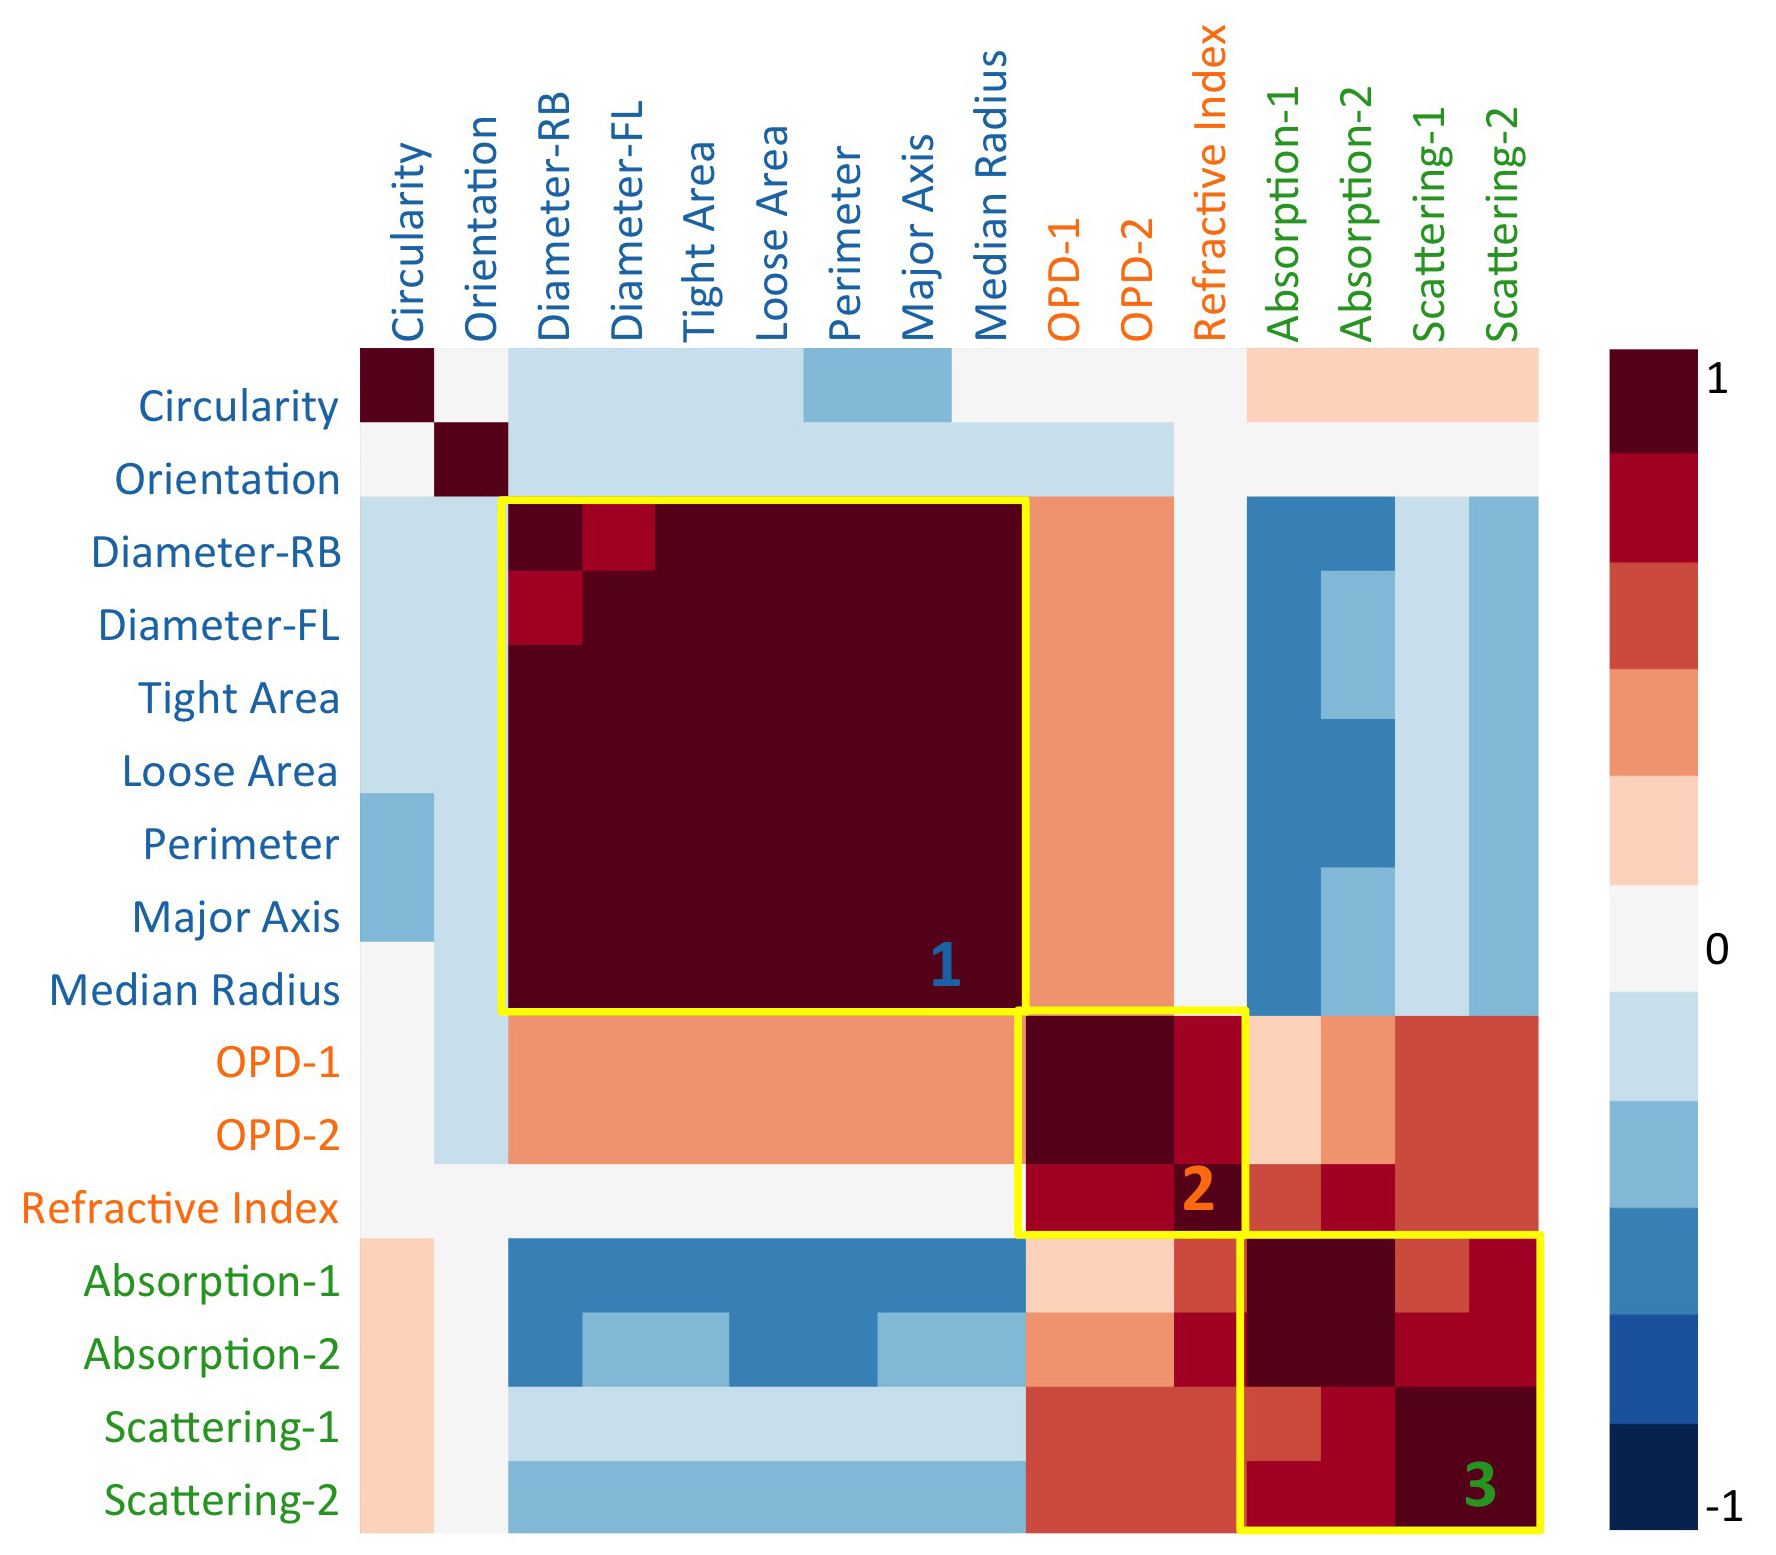
\includegraphics[scale=0.6]{FigureCorrelation.jpg}
\caption{\label{fig:Correlation} Pairwise correlation matrix visualized as a heat map; The map depicts the correlation coefficient between all major 16 features extracted from the quantitative images. Diagonal elements of the matrix represent correlation of each parameter with itself, i.e. the autocorrelation. The subset in box 1, box 2, and box 3 show high correlation because they all measure morphological, optical phase, and optical loss features, respectively. This suggest that the dataset can be adequately represented by a smaller set that excludes highly correlated parameters.}
\end{figure*}

In order to rank the physical features according to their utility in classification, we performed one dimensional classification using each of the 16 features extracted from phase contrast images. Fig.~\ref{fig:FeaturesRank} shows classification accuracy for each feature arranged in descending order. The features are color coded into three categories: morphology, optical phase, and optical loss, to describe the type of information provided by each. The figure provides valuable insight into the relative importance of each category of cell parameters and suggests that morphological information provide the most information about cells but at the same time significant additional information is contained in optical phase and loss measurements. As we will see later in this paper, these conclusions are also supported by results of hyperdimensional classification.

\begin{figure*}
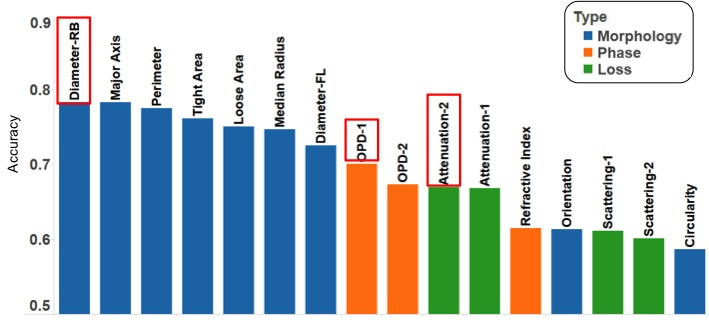
\includegraphics[scale=0.55]{FigureFeaturesRank.jpg}
\caption{\label{fig:FeaturesRank} Ranking of biophysical feature performance based on the accuracy in 1-D classification; The value is the area under receiver operating characteristics curve of each individual parameter. Blue bars show performance of the morphological parameters, which includes diameter along the interrogation rainbow, diameter along the flow direction, tight cell area, loose cell area, perimeter, circularity, major axis length, orientation, and median radius. As expected, morphology contains most information, but other biophysical features can contribute to improved performance of label-free cell classification. Orange bars show optical phase shift features i.e. optical path length differences and refractive index difference. Green bars show optical loss parameters representing scattering and absorption by the cell. Red boxes show the best performed feature in these three categories.}
\end{figure*}

\subsection{Classification}

Neural network is a bio-inspired learning algorithm that works well in classification via supervised learning when adequate amount of training data is available. The basic artificial neural network can be described as a series of transformations performed on the input data \cite{bishop2006pattern, boddy1994neural}. Shown in Fig.~\ref{fig:NeuralNet}, the network consists of an input layer, output layer producing classification results and hidden layer(s) that map the input to the output. Single layer perceptron is neural network with one hidden layer using step function as activation function. This simple model works well on linearly separable data and becomes the bases of deep learning and cortical processor when extended to multilayer. Different values of weights correspond to different linear classification planes. 

\begin{figure*}
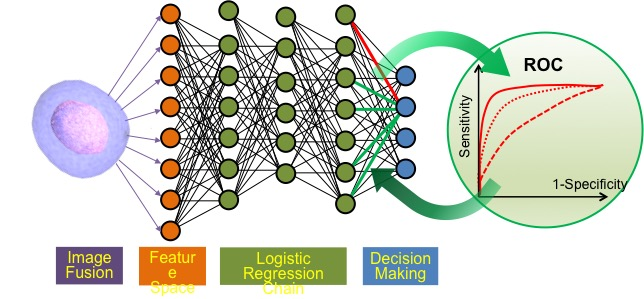
\includegraphics[scale=0.55]{FigureNeuralNet.jpg}
\caption{\label{fig:NeuralNet} Neural network architecture and training via area under the curve (AUC) of the receiver operating characteristics (ROC); Multivariate features of each measurement (cell) are feed into the neural network and the output shows classification labels, i.e. cell types. We train the weights of the last layer perceptron by optimizing the area under ROC curve. Each ROC curve corresponds to a set of weights for connections to an output node, generated by scanning the bias weight. AUC is proven to be statistically consistent and more discriminating than accuracy.}
\end{figure*}

Each layer performs a linear combination on its inputs and performs soft threshold operation on the sum. The output of the node $j$ in layer $l+1$, denoted by $z_j^{(l+1)}$ is generated from inputs $x_1$, $x_2$, \ldots, $x_N$, as
\begin{equation}
\begin{split}
& z_j^{(l+1)} = \h(a_j^{(l+1)}) = \h(\sum_{i=0}^{N_l} \omega_{ji}^{(l)} x_i^{(l)})\\
& i =0,\dotsc,N_l;\quad j=1,\dotsc,N_{l+1};\quad l=1,\dotsc,L-1
\end{split}
\end{equation}
Here $a_j^{(l+1)}$ is the linear combination of inputs, $\omega_{ji}^{(l)}$ are the weights of the linear combination. The summation runs over $N_l$, the total number of nodes in the previous hidden layer, and $L$ is the total number of hidden layers. The function $\h(\cdot)$ is called the activation or hypothesis function and is usually a soft threshold implemented using a logistic sigmoid function $\h(a)=1/(1+\exp(-a))$ or a hyperbolic tangent function. The constant term in the summation, $x_0^{(l)}$, is called the bias.

In classification, there is a trade-off between the sensitivity and specificity. Choosing a low detection threshold (the classifier) results in high sensitivity, however this sacrifices the specificity leading to large number of false positives. To obtain the optimum classifier \cite{powers2011evaluation, liu2008roc}, we use the receiver operating characteristics (ROC) \cite{bradley1997use} and maximize its area under the curve (AUC) \cite{hanley1982meaning, ling2003auc, cortes2004auc, huang2005using} (see inset of Fig.~\ref{fig:OTSWROC}). The ROC is obtained by varying the classification threshold while plotting the True Positive Rate on the vertical axis versus the False Positive Rate on horizontal axis. Therefore, ROC is an ideal tool to visualize the impact of the threshold on classification accuracy. A random guess, corresponding to accuracy of 50\% in binary classification will have an ROC that is a diagonal line. Conversely, a classifier that accurately separates the classes will have an ROC curve that approaches the upper left corner. The AUC parameter measures the area under the ROC curve and serves as an effective metric for optimizing the threshold.

\begin{figure*}
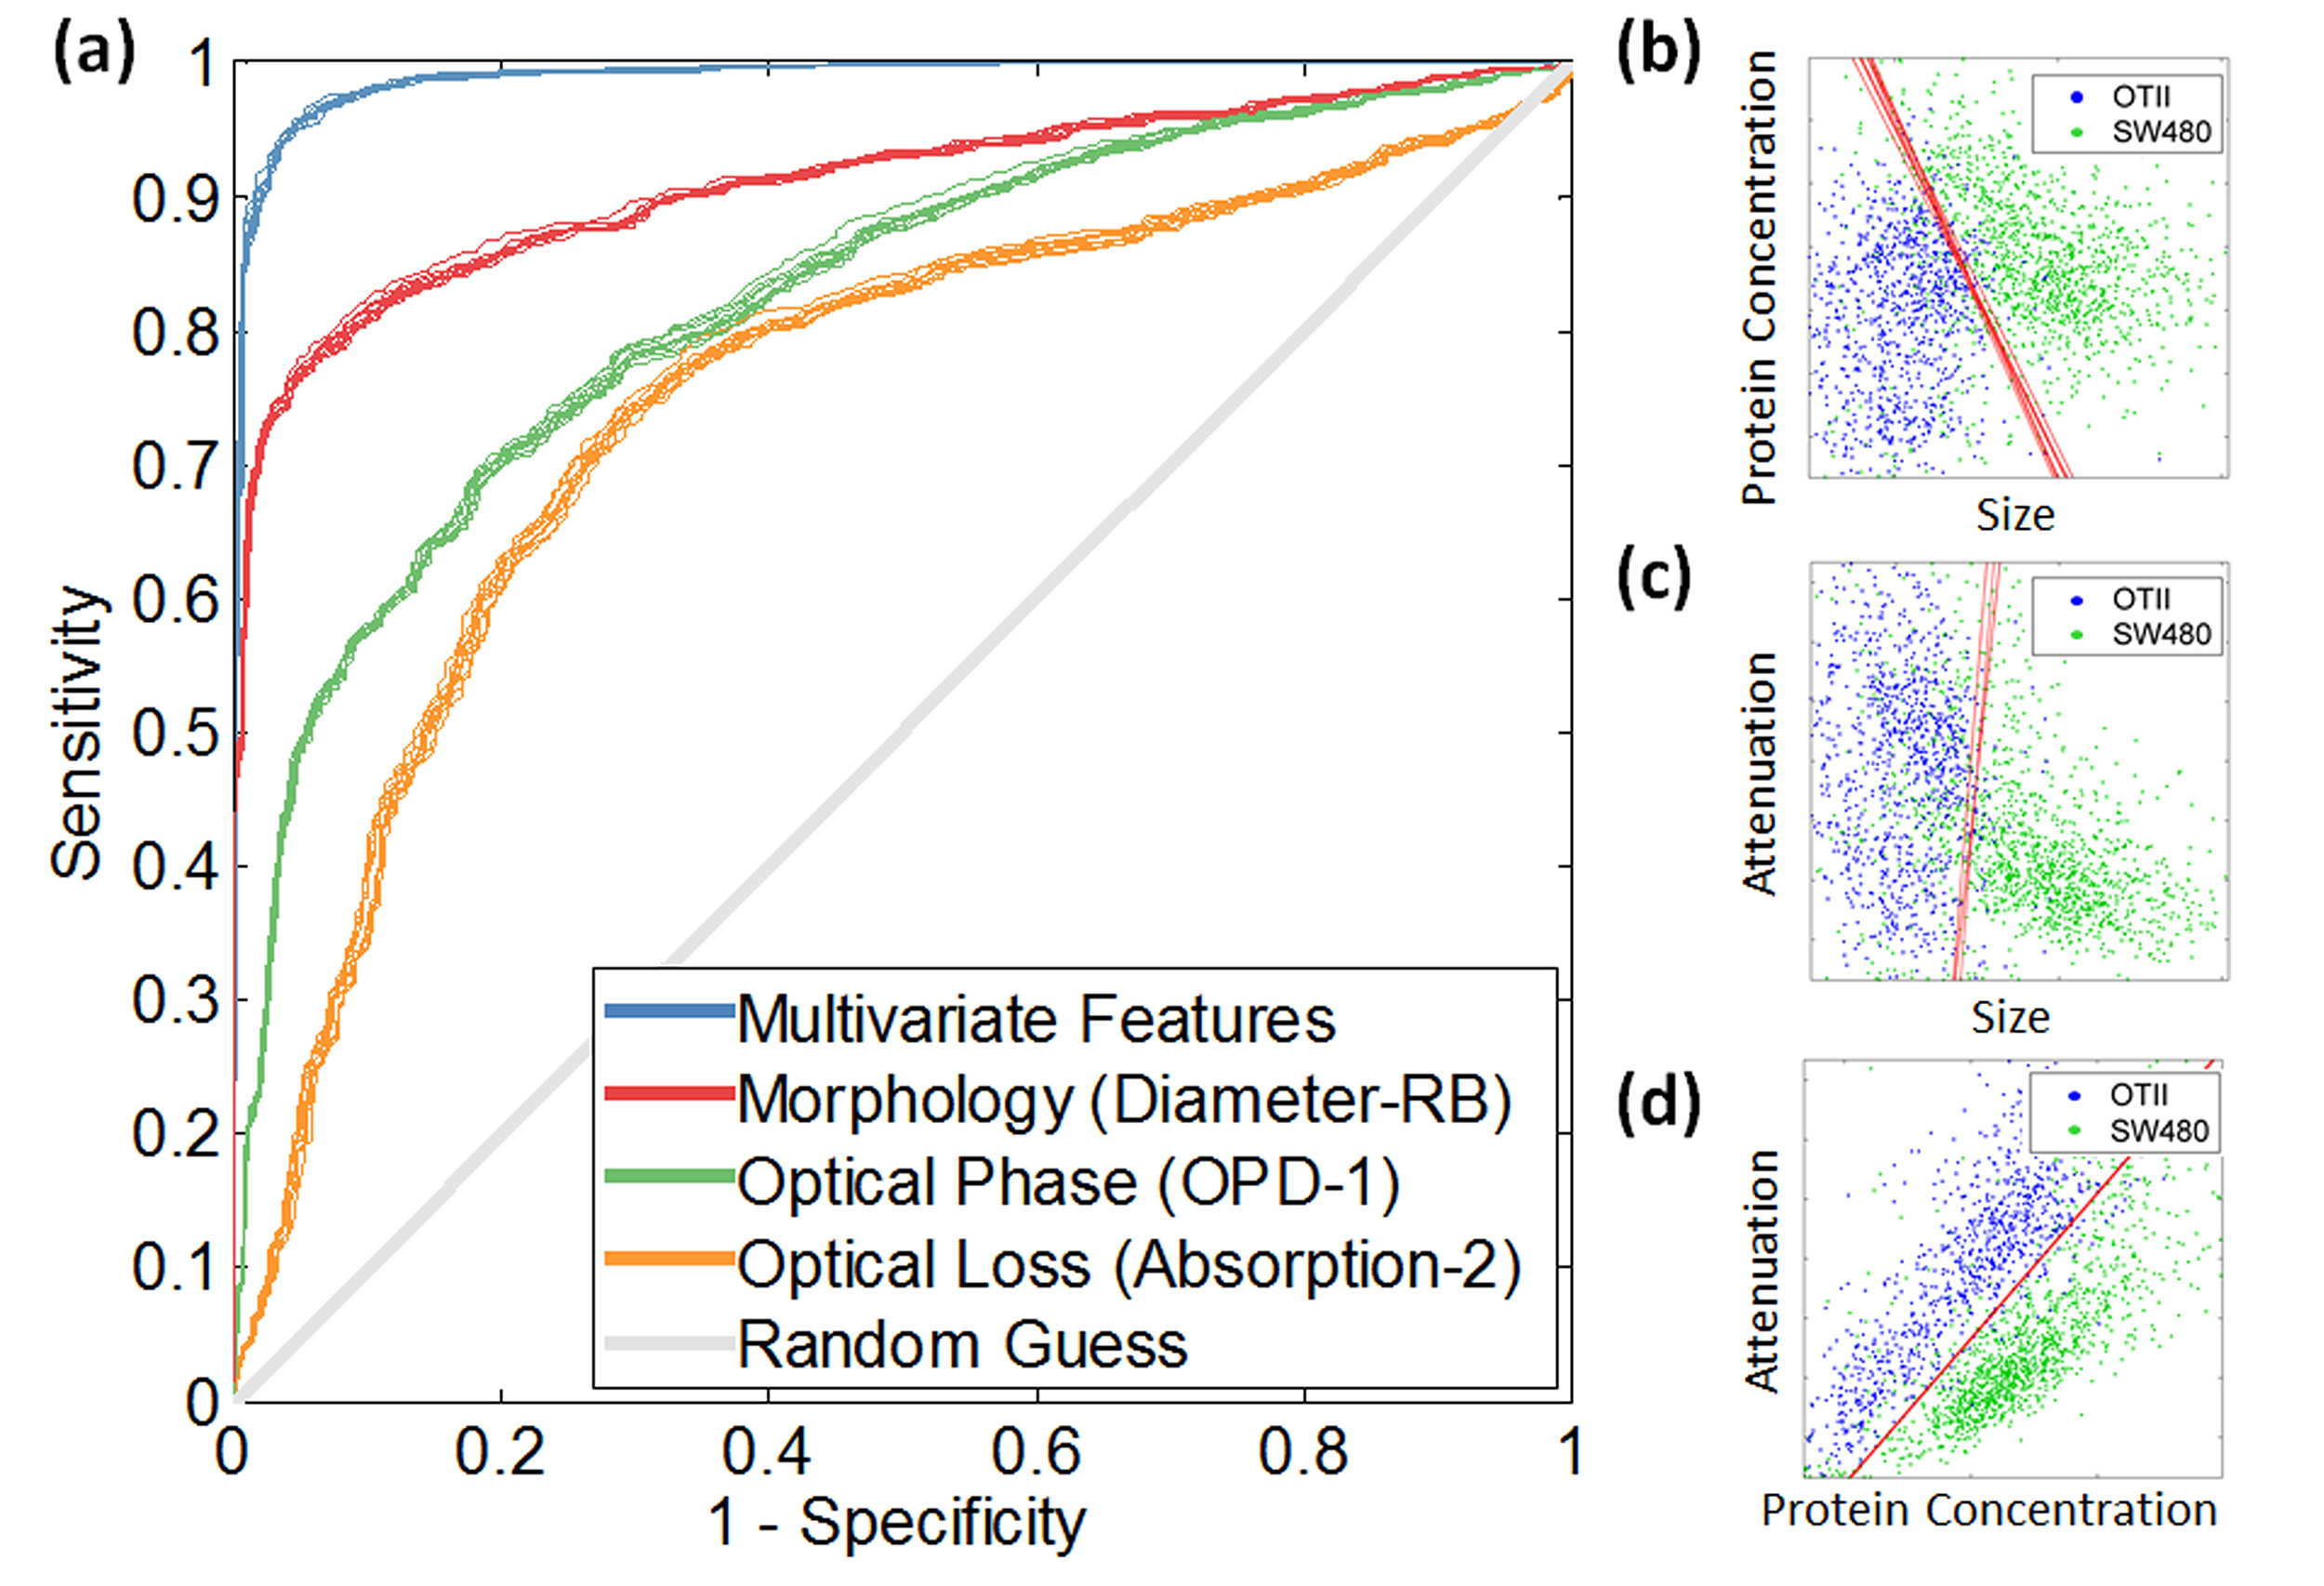
\includegraphics[scale=0.6]{FigureOTSWROC.jpg}
\caption{\label{fig:OTSWROC} Consistency in binary classification of white blood cells (OT-II) and cancer cells (SW-480) by TS-QPI label-free features; (a) For each classifier, we show 10 receiver operating characteristic (ROC) curves demonstrating ten-fold cross validation of the dataset. Blue curves show the classifier performance using all 16 biophysical features extracted from the TS-QPI quantitative images. We also show ROC for classification by three single parameters (red, green, and orange curves) representing the decision performance of the classifiers using only major physical features: diameter (Diameter-RB in Table~\ref{tbl:Features}), optical path length difference (OPD-1 in Table~\ref{tbl:Features}), and absorption (Absorption-2 in Table~\ref{tbl:Features}), respectively. Multivariate analysis based on TS-QPI images (blue curves) shows significant improvement in classification sensitivity and specificity. Additionally, purple curves show the characteristics of the classifier trained with the first dimension in principal component analysis (PCA) feature space after data cleaning. The gray diagonal line shows results of random guess classification. In the ten-fold cross validation, the total data set is split into 10 equal subsets and each time the test is performed for one part while the other nine parts are used for training. The fact that the classifiers remain almost unchanged during the ten runs of cross validation shows consistency and robustness of the dataset and the classifier. (b-d) Decision boundaries (red lines) in two-parameter scatter plots trained by ten-fold cross validation. They also show the consistency and robustness of supervised cell classification by TS-QPI data.}
\end{figure*}

In our work, we use single layer perceptron with AUC as the cost function and genetic algorithm for optimization. This approach of opting for the simpler model, perceptron, as opposed to a multilayer neural network, without compromising the accuracy is consistent with the proverbial ``simpler is better'' known as Occam's Razor \cite{domingos1999role} in the machine learning community. As shown in Fig.~\ref{fig:Correlation} and Fig.~\ref{fig:FeaturesRank}, many of the 16 parameters are correlated and not all measured features in the data set produced by the time stretch quantitative phase imaging have the same amount of information. That result suggests that it may be possible to reduce the 16 dimensional data set to a smaller set of uncorrelated orthogonal dimensions without significantly compromising the classification accuracy. In that spirit, we have used principle component analysis (PCA) for dimensionality reduction. The PCA algorithm finds an alternative lower dimension space such that variance of data projected onto this subspace is maximized along subspace dimensions. By revealing the structure in data that best explains the variance, PCA achieves data compression via dimensionality reduction. 

We have performed PCA on the 16 dimensional data set acquired by our time stretch QPI system. This maps the data from the physical feature space to the PCA space. Fig.~\ref{fig:PCA} shows the percent of the variance in data explained by each component (lower chart). The key observation is that most of the variance can be accounted for by the first two principle components. The upper portion of the plot shows the AUC for binary classification using each of the principle components. Interestingly, the first component with the highest explained variance is not necessarily the most important component for classification. This is not surprising since PCA components are optimized to the variance of data but not to the data labels. Therefore, apriori intuition about the physical significance of the features in the case here, is superior to PCA in eliminating dimensions that do not provide high value in classification. Nevertheless, in situations where physical intuition about meaning of features does not exist, PCA is a valuable tool. A second observation is that principle components that have low explained variance do have some value in classification. 

\begin{figure*}
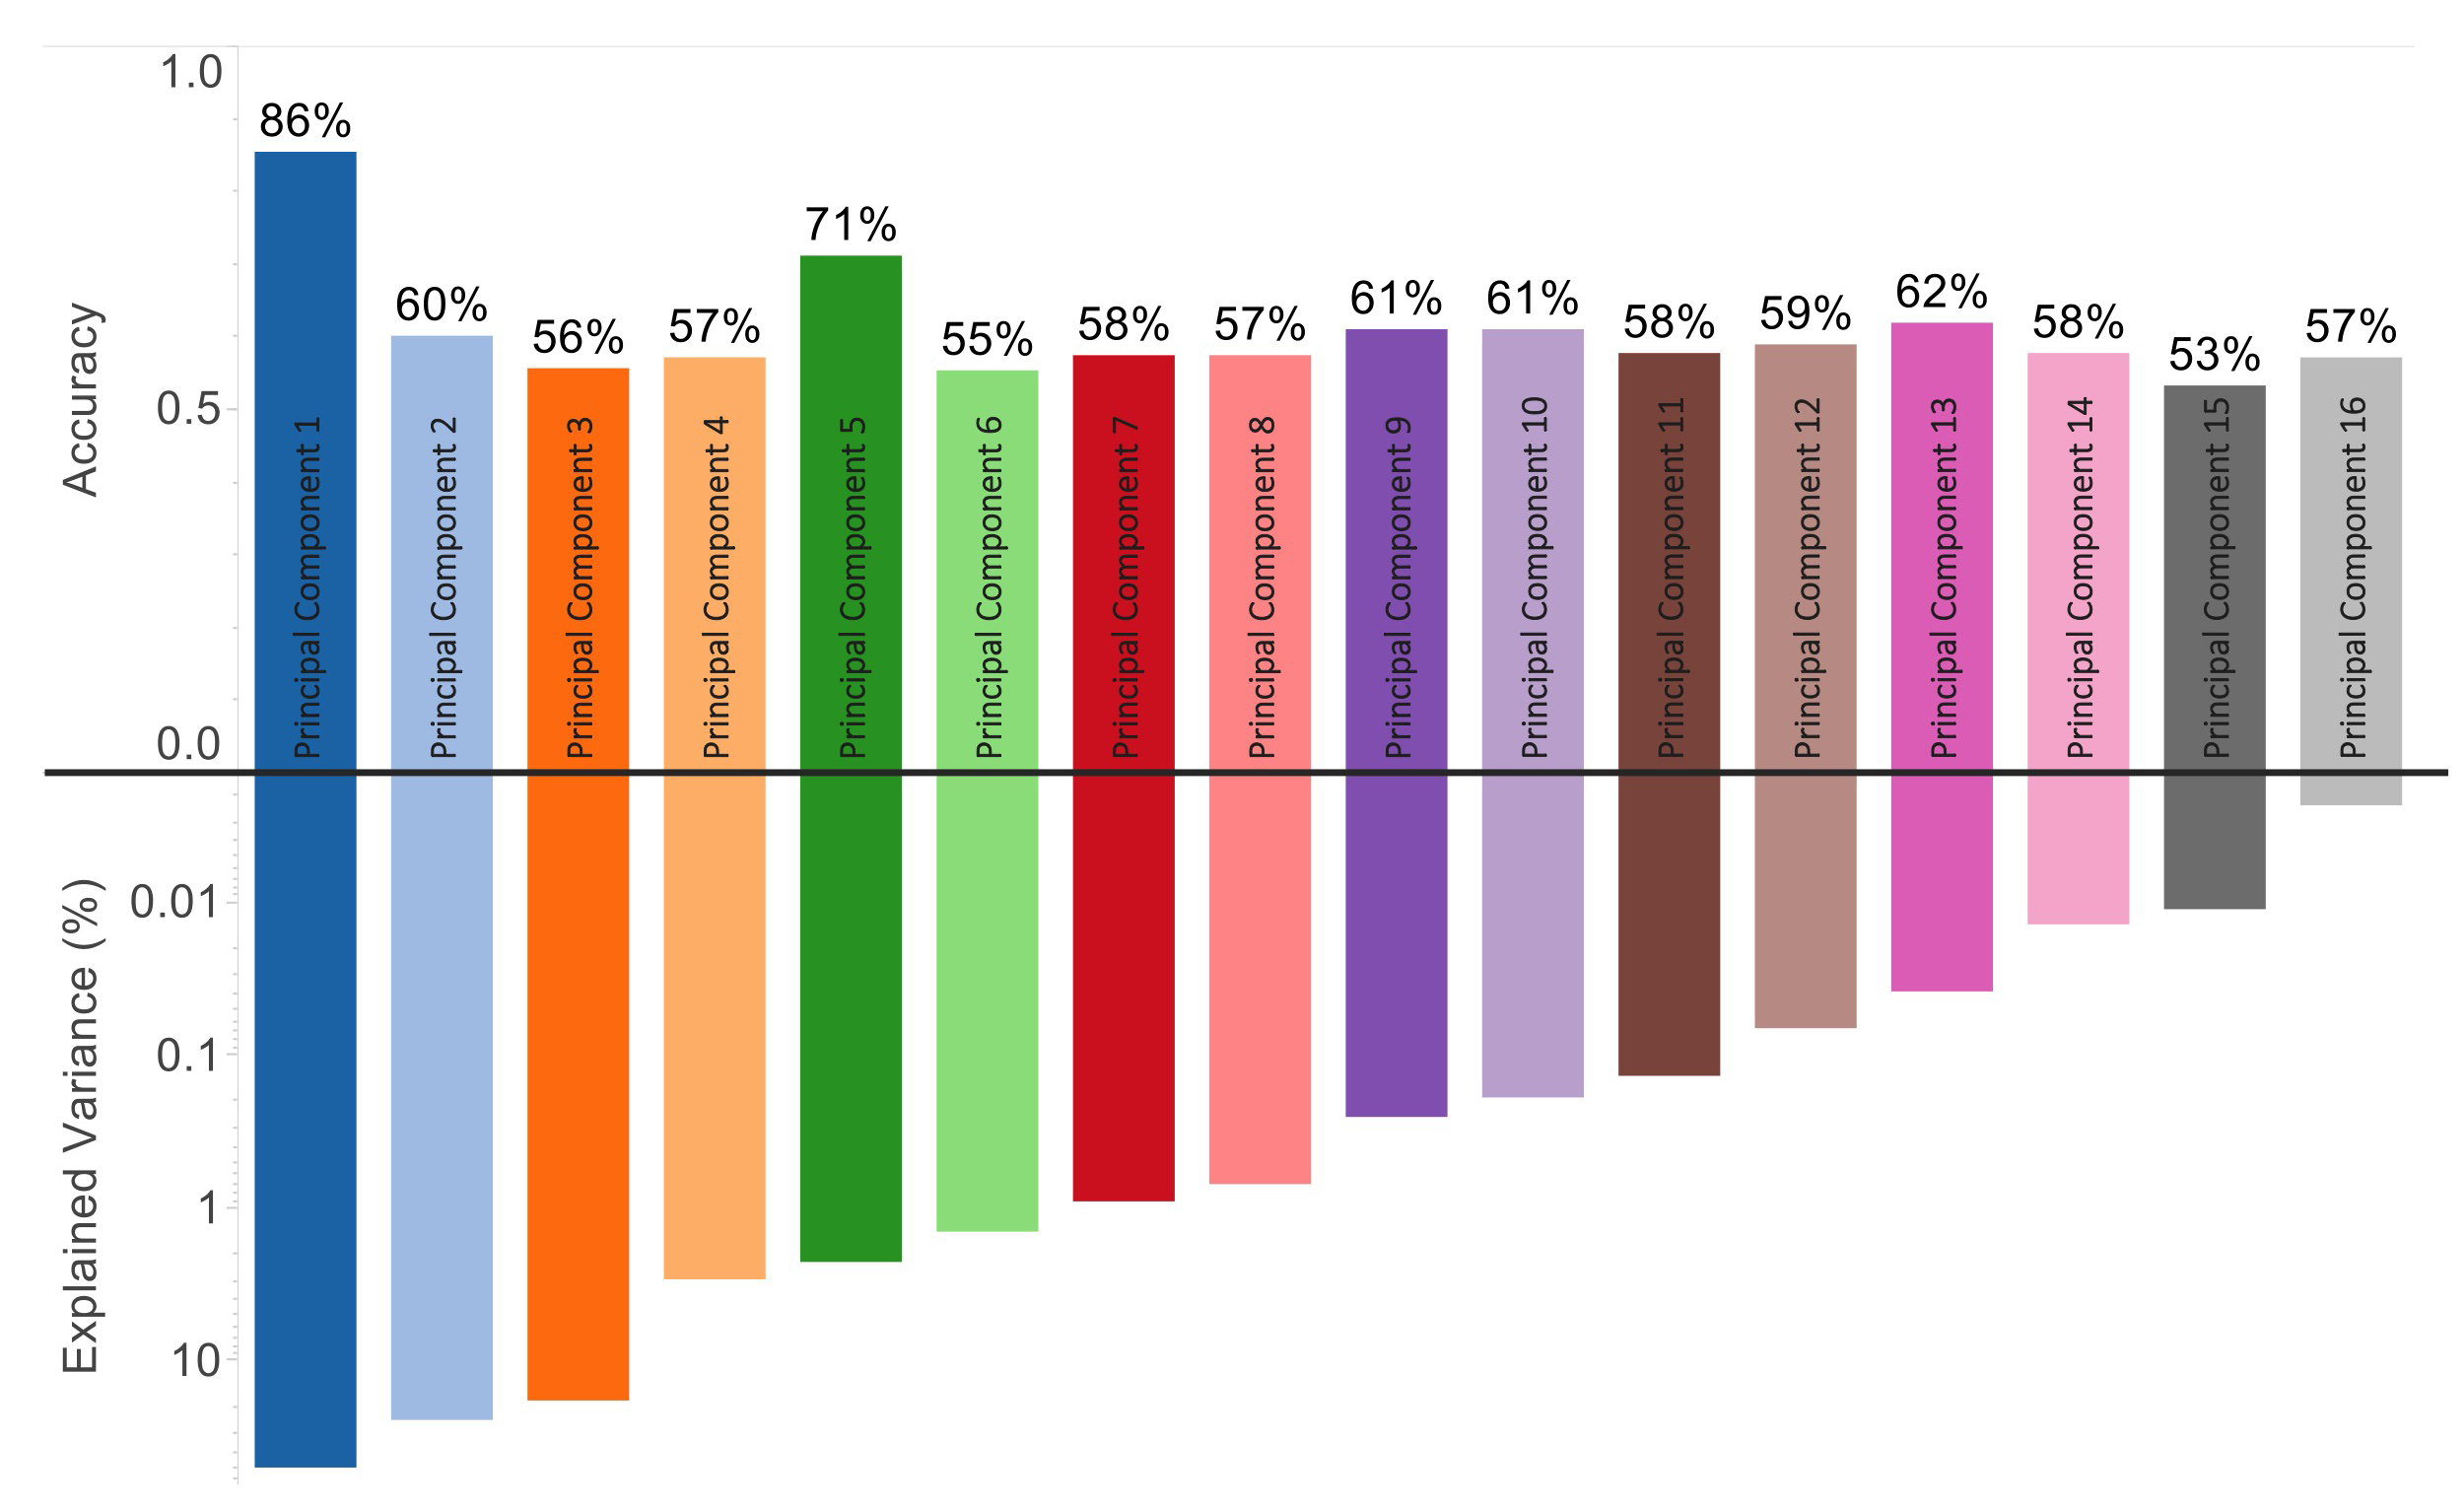
\includegraphics[scale=0.55]{FigurePCA.jpg}
\caption{\label{fig:PCA} Principal component analysis (PCA); Performance ranking of individual principal components in PCA space. The height of each bar shows the percentage of the total variance explained by each principal component, accounting for the variability expressed in the data. Reasonably, principal components with larger variability do not necessarily give high accuracy in classification.}
\end{figure*}

To optimize the classifier performance in neural networks, cross entropy and mean squared error are typical cost functions used. In this work, we use the ROC as the cost function to train the neural network because it considers the balance between the sensitivity and specificity of the classification [Hanley 1982]. AUC has been proven to be advantageous to the mean square error for evaluating learning algorithms \cite{verrelst1998use} and minimizing the error rate may not lead to the best possible AUC values [Yan 2003, Cortes AUC optimization, Huang AUC].Here we use single layer perceptron but trained by globally maximizingthe area under the ROC curve (AUC). By varying the bias and the weights, the offset and slope of the classifier is scanned, respectively. To speed up the computation for high dimensionality analysis, we employ genetic algorithm. 

\subsection{Demonstration in Classification of OT-II and SW-480 Cells}

Classification of cells based on size alone in a label-free manner has been previously reported by several groups [Vona et al, others]. However, in contrast to these single parameter (size) approaches, our multi-parameter classification, enabled by the time stretch QPI, offers considerable improvements in detection sensitivity and accuracy for cancer diagosis and selection of algal species. To demonstrate the effectiveness of the machine learning plus time stretch QPI imaging system for cancer cell detection, we used OT-II hybridoma T cells as a model for normal white blood cells and SW-480 colon cancer cells. A 16 feature data set was measured using the imaging system and feature extraction technique described previously. By sliding the detection limit along the direction perpendicular to the optimum classification plane, a receiver operating characteristic (ROC) curve for multi-dimensional data is generated (Fig.~\ref{fig:OTSWROC}).

Blue curves in Fig.~\ref{fig:OTSWROC} show the ROC for classification using all sixteen biophysical features extracted from the time-stretch QPI images. The grey diagonal line shows a random guess classifier with no discrimination skill. For generating the ROC curves, we employ the normal unit vector of a decision boundary in n-sphere and use genetic algorithm for optimization. At step k+1 a trial set of weights (children) is randomly generated in the neighborhood of the present set (parents). Each generation produces new ROC curves. The genetic algorithm randomly selects from this population and uses them as parents to produce the children for the next generation by mutation and crossover. Over successive generations, the population evolves toward an optimal solution that maximizes the AUC. The area under the ROC curve (AUC) was calculated using a non-parametric method based on constructing trapezoids under the curve.

As a way to visualize the improvement in classification by hyperdimensional feature space of TS-QPI, we also show the ROC curves of classification based on several single features: diameter along the interrogation rainbow, integral of cell's optical path length difference, and cellular absorption in near-infrared window. These three biophysical parameters individually perform the highest accuracy among morphology, optical phase, and optical loss parameter groups respectively. But multivariate analysis based on TS-QPI shows significant improvement in classification. For each type of classification we show the ROC for 10 fold cross validation data set. As the curves approach random guess line, the 10 fold cross validation curves deviate more from each other. Additionally purple curves shows the classifier optimized with the first principal component in PCA feature space.

\subsection{Demonstration in Algae Lipid Content Classification}

Microalgae are considered one of the most promising feedstock for biofuels \cite{merchant2012tag}. The productivity of these photosynthetic microorganisms in converting carbon dioxide into useful carbon-rich lipids greatly exceeds that of agricultural crops [insert reference]. Worldwide, research and demonstration programs are being carried out to develop the technology needed to expand algal lipid production as a major industrial process. Selecting high yield microalgae with fast growth factors are essential in biofuel production industry. Because algae differ greatly in size and structure, cell size alone provides insufficient information for cell classification. Here we show that adding optical phase and loss data, obtained by the phase contrast time stretch imaging flow cytometer, to size data enables cells to be distinguished on the basis of lipid content. 

To test our apparatus for its ability to separate high and low-lipid containing cells we exploited the starch-null \textit{STA6} strain of Chlamydomonas. This strain is deleted for \textit{STA6} \cite{zabawinski2001starchless} (encoding the small subunit of ADP-glucose-pyrophosphorylase), and when nitrogen-deprived accumulates more lipid than wild-type \cite{work2010increased, li2010chlamydomonas, goodenough2014path, blaby2013systems}. Comparison of the two strains therefore provides an ideal setup to test our ability to distinguish lipid-content phenotypes.

Fig.~\ref{fig:AlgaeScatter}a shows the 3D scatter plot showing the three principle physical features for the two algae populations. Also shown is the scatter plot obtained using a conventional flow cytometer. It is readily apparent that the TS-QPI capture much more information about individual cells and is better suited for differentiation of low- and high-lipid content algae species. In Fig.~\ref{fig:AlgaeScatter}b, we show ROC curves for binary classification of these populations. Blue curve shows the classifier performance using all 16 physical features extracted from the time-stretch QPI images. Red, green, and orange curves show the classifier decision made using only the three major biophysical features: diameter for morphology (Diameter-RB in Table~\ref{tbl:Features}), optical path length difference for optical phase (OPD-1 in Table~\ref{tbl:Features}), and absorption for optical loss (Absorption-2 in Table~\ref{tbl:Features}). Additionally, we show ROC curves in purple for classification based on the first principal components in PCA space. We observe that while biophysical parameters, in particular cell diameter, is an effective feature for classification, hyperdimensional classification using all 16 parameters offers the best accuracy. 

\begin{figure*}
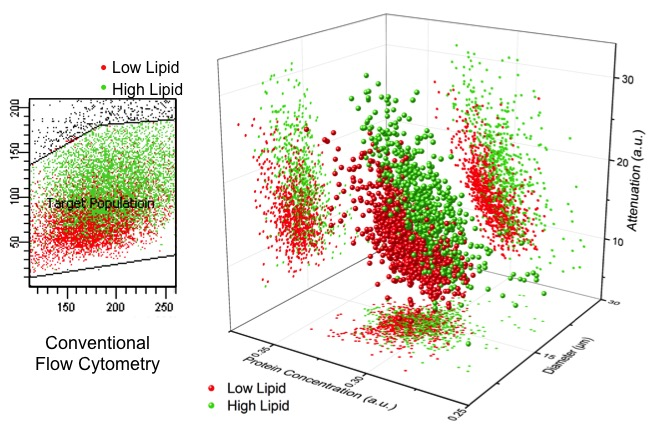
\includegraphics[scale=0.5]{FigureAlgaeScatter.jpg}
\caption{\label{fig:AlgaeScatter} Classification of algae cells (Chlamydomonas reinhardtii) based on their lipid content by TS-QPI; (a) Three-dimensional scatter plot based on size, protein concentration, and attenuation of the cells measured by TS-QPI, with 2D projections for every combination of two parameters. Inset: Conventional label-free flow cytometry using forward scattering and side scattering is not enough to distinguish the difference between high-lipid content and low-lipid content algae cells. Time-stretch QPI is much more effective in separating the two algae populations. (b) ROC curves for binary classification of normal and lipid-rich algae species using ten-fold cross validation; blue curve shows the classifier performance using all 16 biophysical features extracted from the TS-QPI quantitative images. Red, green, and orange curves show the classifier decision performance using only the three major physical features: diameter (Diameter-RB in Table~\ref{tbl:Features}), optical path length difference (OPD-1 in Table~\ref{tbl:Features}), and absorption (Absorption-2 in Table~\ref{tbl:Features}), respectively. Additionally, we show ROC curves in purple for classification based on the first principal components in PCA space. The diagonal line shows results of random guess classification. Clearly, the label-free cell classification performance improves as more biophysical features are employed.}
\end{figure*}

\section{Conclusion}

Time-stretch quantitative phase imaging (TS-QPI) is capable of capturing images of flowing cells with minimal motion distortion at unprecedented rates of 100,000 cells/s. TS-QPI relies on spectral multiplexing to capture simultaneously both phase and intensity quantitative images in a single measurement, generating a wealth of information of each individual cell eliminating the need for labeling with undesirable biomarkers. Here, we summarized the information content of these images in a set of 16 parameters for each cell, and performed classification in the hyperdimensional space of this dataset. Our classifier learning method is based on evolutional optimization of the area under the receiver operating characteristic curve for a single-layer binary-classifier neural network. The results from two experimental demonstrations, one on detection of cancerous cells among white blood cells, and another one on identification of lipid-rich algae, shows that classification accuracy by using the TS-QPI hyperdimensional space is more than 17\% better than the conventional size-based techniques.

\section{\label{scn:Methods} Methods}

\subsection{Time Stretch Quantitative Phase Imaging (TS-QPI) System}

Broadband optical pulses from a mode-locked laser (center wavelength = 1565 nm, repetition rate = 36.128 MHz, pulse width ~ 100 fs) are further broadened using a highly nonlinear fiber to approximately 100 nm with a spectral range up to 1605 nm. These broadband pulses are then linearly chirped to 1.2 ns pulse width by a short dispersion compensating fiber (DCF) of 60 ps/nm, so that an erbium doped fiber amplifier (EDFA) can amplify them with minimal distortion. A coarse wavelength division multiplexer (WDM) filters the pulses from 1581 nm to 1601 nm, where the spectrum is reasonably flat. Therefore, the total bandwidth of the pulses interrogating the cells in our setup is less than 20 nm centered at 1591 nm, giving a negligible fractional bandwidth of 1.3\%. These filtered pulses then pass through an optical circulator and are coupled to free-space with a fiber collimator.

Free-space laser pulses were linearly polarized with quarter- and half-wave plates, and then spatially dispersed with a pair of reflection diffraction gratings, so that each wavelength component of the collimated beam was positioned at a different lateral point similar to a line flash rainbow. A beam reducer shrank the rainbow beam 6 times with a pair of 90 degree off-axis parabolic gold-coated mirrors with reflected focal lengths as 152.4 mm and 25.4 mm, respectively. Next, a 15 degree off-axis parabolic gold-coated mirror with 635 mm reflected focal length and a long working-distance objective lens with 0.4 numerical aperture further shrank the rainbow to about \SI{130}{\micro\meter} in width, i.e. field of view. Reflective optics with parabolic gold-coated mirrors is used in our experimental demonstration to minimize loss, aberration, and polarization sensitivity. The rainbow flashes were then split into the two arms of a Michelson interferometer by a beam splitter. In the sample arm, the rainbow pulses pass through the cells and are reflected by the reflective substrate of the microfluidic device. In the reference arm, a dielectric mirror reflected the rainbow with a length mismatch with the sample arm causing 5 GHz interference fringes. Cells are hydrodynamically focused at the center of the channel flow at a velocity of 1.3 m/s. The reflected pulses from reference and sample arms were recombined at the beam splitter, compressed by the two diffraction gratings and coupled back into the fiber. These return pulses were spectrally encoded by the spatial information of the interrogation field of view. Then they were redirected by the optical circulator to a Raman-amplified time-stretch dispersive Fourier Transform (TS-DFT) system followed by a 10 Gb/s photodetector (Discovery Semiconductors DSC-402APD). An analog-to-digital convertor (Tektronix DPO72004C) with a sampling rate of 50 GS/s and 20 GHz bandwidth is used to acquire the output signal of the photodetector.

\subsection{Coherent Detection and Phase Extraction}

Unlike in conventional heterodyne detection, which uses a narrow band continous-wave beam as the local oscillator, the coherent detection in our time stretch system uses an unmodulated copy of the original optical input, which is a broadband chirped optical pulse \cite{buckley2013coherent, devore2014coherent}. 

The input optical signal is split into two arms of the Michaelson Interferometry at the beam splitter. The one in sample arm, $E_s(t)\exp(i\omega_s t)$, passes through the object, and then, is combined with the other one from the reference arm $E_{LO}(t)\exp(i\omega_{LO} t)$. $E_s(t)$ and $E_LO(t)$ are the electric field amplitudes of the sample and reference sources, and $\omega_s$ and $\omega_{LO}$ are the optical frequencies of sample and reference fields, respectively. Not only the electric field amplitude after passing through semitransparent objects, $E_s^\prime(t)$, will be modulated by the optical absorption and scattering in the sample arm, but also the optical path length difference will lead to a phase shift, $\Delta\varphi(x,t)$, inducted by refractive index change along the interrogation beam. Thus the combined electrical field is
\begin{multline}
E_{total}(t) = E_s^\prime(t) \exp \lbrace i[\omega_s t+\Delta\varphi(x,t)] \rbrace\\
+ E_{LO}(t) \exp(i\omega_{LO} t)
\end{multline}
In our case, $E_{LO}(t)$, as a local oscillator (LO), is same as $E_s(t)$ but with reduced power. After time stretch, the frequency components in $\omega_s$ and $\omega_{LO}$, are mapped into time. That is, electric field detected at time t is one-to-one mapped from frequency domain,
\begin{multline}
E_{total}(t) = E_s^\prime(t_p,\omega_s) \exp \lbrace i[\omega_s t+\Delta\varphi(x,t)] \rbrace\\
+ E_{LO}(t_p,\omega_{LO}) \exp(i\omega_{LO} t)
\end{multline}
where $t_p$ corresponds to the $p$-th incoming pulse. Note that $E_s(t_p,\omega_s)$ can be simplified as $E(\omega_s)$ when pulse shape (magnitude of each wavelength) is stable from pulse to pulse.

$\omega_s$ detected at $t$, is mixed with local oscillator $\omega_{LO}$ at $t$, which is a copy of $\omega_s(t)$ within the same pulse but delayed by $\Delta\tau$,
\begin{equation}
\omega_{LO}(t) = \omega_s(t-\Delta\tau)
\end{equation}
where $\Delta\tau = 2 \Delta L/c$ is the delay mismatch in Michaelson interferometry and $\Delta L$ is the length mismatch in the two arms. Define $t_i$ as the relative time within each pulse,
\begin{equation}
\begin{split}
E_{LO}(t_p,\omega_{LO}) &= E_{LO}(t_p,\omega_{LO}(t_i)) \\
&= E_s(t_p,\omega_s(t_i-\Delta\tau))
\end{split}
\end{equation}
Since the difference in arrival times at the photodetector after time stretch between each frequency component of reference and sample signals is same as the delay difference in interferometry arms, $\Delta\tau$, the beating frequency or modulation frequency of the interference fringes is
\begin{align}
\omega_f & = \omega_s(t_i ) - \omega_{LO}(t_i ) = \omega_s(t_i ) - \omega_s(t_i-\Delta\tau)\\
& \approxeq \frac{2\pi c}{\lambda_c^2} (\lambda(t_i) - \lambda(t_i-\Delta\tau))\\
& = \frac{2\pi c}{\lambda_c^2} \cdot \frac{\Delta\tau}{\beta L_f} = \frac{4\pi\Delta L}{\lambda_c^2 \beta L_f}
\end{align}

where $\lambda_c$ is the central wavelength, $\beta$ is the group velocity dispersion, and $L_f$ the length of dispersive fiber. Thus the energy flux absorbed at the photodetector, is proportional to the product of the sum of the electric fields
\begin{multline}
I_{PD}(t) \propto \lvert E_s^\prime(t_p,t_i) \rvert^2 + \lvert E_s(t_p,t_i-\Delta\tau) \rvert^2\\
+ 2 \operatorname{Re}\lbrace E_s^\prime(t_p,t_i) \cdot E_s^*(t_p,t_i-\Delta\tau)\\
\cdot \exp[i(\omega_f t + \Delta\varphi(x,t))] \rbrace
\end{multline}
where the asterisk signifies complex conjugation, and $\operatorname{Re}$ is the real part. Note that high frequency terms are averaged over time as it is far beyond the photodetector response time. 

Thus the time stretched temporal waveforms corresponding to each line scan image consists of two features \cite{mahjoubfar2014label}. One is $\rvert E_s^\prime(t_p,t_i) \lvert^2 + \rvert E_s(t_p,t_i-\Delta\tau) \lvert^2$, a temporal envelope of the time-stretched optical pulse usually at baseband frequencies. The amplitude of this envelope corresponds to the temporal shape of the optical pulse and its deviations caused by the object as in brightfield microscopy. It provides information about optical loss, i.e. light absorption and scattering caused by surface roughness, granularity, and inner cell organelle complexity. The other feature is $I_PD^{(f)} = 2 \operatorname{Re}\lbrace E_s^\prime(t_p,t_i) \cdot E_s^*(t_p,t_i-\Delta\tau) \cdot \exp[i(\omega_f t + \Delta\varphi(x,t))] \rbrace$, a fast oscillating fringe, caused by the interference of the linearly chirped pulses multiplexed between the sample and reference arms in the Michelson interferometer.

The second feature, $I_{PD}^{(f)}$, containing only spectral features modulated at $\omega_f$ is separated by a band-pass filter to extract the object phase shift, $\Delta\varphi(x,t)$. The instantaneous phase of this feature can be readily retrieved from its analytic representation given by Hilbert transform, $\hilbert$:
\begin{align}
\angle I_{PD}^{(f)} &= \omega_f t + \Delta\varphi(x,t) \\
&= \arg[I_{PD}^{(f)} (t_p,t_i ) + j \cdot \hilbert(I_{PD}^{(f)}(t_p,t_i))]
\end{align}
Here $\arg$ means the argument of a complex number. A one-dimensional phase unwrapping algorithm followed by background phase removal gives the object phase shift, 
\begin{equation}
\Delta\varphi(x,t) = \unwrap(\angle I_{PD}^{(f)}) - \omega_f t
\end{equation}
The unwrapping algorithm used in our processing acts when the absolute phase difference between two consecutive samples of the signal is greater than or equal to $\pi$ radians, and adds multiples of $2\pi$ to the following samples in order to bring the consecutive samples phase difference in the acceptable range of $-\pi$ to $\pi$.

\subsection{Image Reconstruction}

We reconstruct both quantitative brightfield and phase-contrast images simultaneously from single-shot frequency-multiplexed interferometric measurements. The envelope and phase of the time-domain signal $I_PD (t_i,t_d)$ was firstly mapped into series of spatial information $I_{PD}(t_i,x_j)$, forming a line scanning brightfield image and phase contrast image, illuminated by the optical pulse at time $t_i$ (Fig.~\ref{fig:2DImage}b). This is because within each optical pulse, the spatial information is mapped one-to-one into spectral domain, $x_j \rightarrow \lambda_j$, and spectrum is stretch in time, $\lambda_j \rightarrow t_d^{(i)}$, where $t_d^{(i)}$ is the relative group delay time of each frequency component within a pulse with respect to the central wavelength. These line-scan images based on $I_{PD}(t_1,x)$, $I_{PD} (t_2,x)$, $I_{PD} (t_3,x)$, \ldots were then cascaded into a two dimensional image corresponding to $I_{PD}(y,x)$, where the second dimension $y$ is the spatial mapping of time elapse based on object flow speed. 

The optical path length difference image can be formed by the phase shift line scans as
\begin{equation}
OPD(x,y) = \frac{\lambda(t_i,t_d)}{2\pi} \Delta\varphi(x,t) = \frac{\lambda(x,y)}{2\pi} \Delta\varphi(x,y)
\end{equation}
On the other hand, if the axial thickness of the cell at reconstructed image pixel $(x,y)$ is $d(x,y)$,
\begin{equation}
OPD(x,y) = 2 [n_{cell}(x,y) - n_{solution}(x,y)] \cdot d(x,y)
\end{equation}
in which $n_{cell}$ and $n_{soluiton}$ are the refractive indices of the cell and the surrounding buffer solution, respectively. The factor 2 is to account for the fact that each wavelength component passes the cell twice in Michelson interferometer. 

If we integrate Eq. (5) over the area of the cell, we can derive an average refractive index contrast for the cell, which corresponds to the average protein concentration of the cell:
\begin{equation}
\overline{\Delta n_{cell}} = \overline{n_{cell} - n_{solution}} = \frac{\iint_{cell} OPD(x,y) dx dy}{2 V}
\end{equation}
where $\iint_{cell} t(x,y) dx dy$ is the volume of the cell obtained from its diameter, $d$, as $V \approx \pi d^3/6$. 

The combined absorption and scattering coefficients (attenuation coefficient) of each cell corresponding to the intensity variations (optical loss) induced by the cell is obtained from the amplitude of the slowly varying envelope feature of the interferogram as
\begin{equation}
\Delta I = \frac{I_{PD}(t_i,t_d)}{I_{PD}(t_{background},t_d)}
\end{equation}
where $t_{background}$ corresponds to a measurement (an interrogation time) that there is no cell in the field of view, and only the background pulse shape is captured. 

\subsection{Big data analytics pipeline}

The high-content image analysis and cell screening pipeline is implemented by combining multiple informatics tools, namely CellProfiler for image processing \cite{carpenter2006cellprofiler,kamentsky2011improved}, MySQL/MangoDB for database, Matlab for machine learning, and Javascript for interactive visualization. 
Feature extraction from quantitative phase and intensity images leads to multiplexed hyperdimensional analysis. When monitoring a large amount of cells, it is not initially trivial which features are statistically significant for cell classification. However, once the learning is performed, a ranking of the significance of the parameters can be helpful for future tasks on the same type of samples. 

In our pipeline first of all, image noise reduction and smoothing have been performed. Smoothing can remove artifacts that are smaller than optical resolution limit. Then for object segmentation, which is one of the most challenging steps in image processing and highly influences the downstream classification, we use the Otsu's thresholding method. Since the ratio of the number of foreground (objects or cells) pixels to that of the background pixels is small, and it normally does not vary substantially from image to image), the histogram of pixel gray levels is fitted into two classes,  corresponding to the background and foreground pixels. The optimum threshold is calculated so that the total weighted variance within both classes is minimized or intra-class variance is maximized. Once objects are identified in the image, morphology of each single cell can be described by area, diameter, uniformity, aspect ratio, perimeter, number of surrounding clumped cells, etc.

The capability to identify clumped cells from single large cells greatly reduces the misclassification rate in imaging flow cytometry compared to traditional flow cytometry. Intensity peaks of pixel brightness within each object are used to distinguish clumped objects. The object centers are defined as local intensity maxima in the smoothed image. Retaining outlines of the identified objects helps validate and visualize the algorithm. In the next step, we discard the objects touching the borders of the image, i.e., the edges of the field of view and data acquisition time window. However, the chance of cells showing up at the edges is very low due to hydrodynamic focusing. We are also capable of excluding dust, noise, and debris by neglecting the objects that are too small or their aspect ratio is too extreme to be a cell. Size measurements are performed along both the rainbow direction and the cell flow direction. Measurement of the diameter along the rainbow direction is primarily used for cell classification since it helps to eliminate measurement inaccuracies caused by fluctuations of flow speed. 

The intensity variations caused by cell absorption and scattering can be extracted from the pixel intensities in the brightfield images, and the phase shift caused by the cell protein concentration can be extracted from the pixel intensities in the phase contrast images. Due to limited optical resolution of the setup, the edges of bead or cell are blurred, generating the tails of point spread functions in phase and intensity signals outside of the diameter boundaries. In order to maximize the accuracy in morphological, phase, and loss measurements, after object segmentation, we expanded the object boundaries (Fig.~\ref{fig:2DImage}, orange circles) by 2.5 um (optical resolution of the setup measured by knife-edge method), which serve as loose boundaries, indicating the area within which the pixel intensities are measured and integrated in phase and transmission images (Fig.~\ref{fig:2DImage}, green circles).

To calculate the refractive index, the axial diameter along the interrogation optical beam is assumed to be equal to the lateral diameter along the rainbow direction, since cells in suspension relax to a spherical shape due to surface tension.

\subsection{Calibration of size measurement}

To calibrate the imaging system and image processing pipelines for size measurement, \SI{5}{\micro\meter} polystyrene beads (from Polysciences, Inc.) with NIST traceable particle size standards were analyzed. Size measurement of the polystyrene beads had a distribution with \SI{5.06}{\micro\meter} expected mean and \SI{0.5}{\micro\meter} standard deviation. The broadened standard deviation was within the range of optical resolution limit and was caused mainly by performing object recognition on resolution limited images.

In comparison, phase shift images are robust and insensitive to axial defocusing \cite{spadinger1990effect} caused by the limited depth-of-focus of the objective lens and alignment of the cells determined by the microfluidic channel structure. Any unscattered photon that passed through the cellshas the chance to be influential in phase images. This makes the size measurement in phase shift images relatively accurate and consistent. 

\subsection{Data cleaning}

Data cleaning includes two steps. Firstly, Hotelling's T-squared distribution is calculated and top 2\% of the extreme data was set as outliers due to experimental errors or object recognition errors. Secondly, debris discrimination is performed; any data point with negative phase shift was considered as either air bubble, flow turbulence, or object recognition errors.

\subsection{Microfluidic channel design and fabrication}

The PDMS microfluidic channel is custom-designed so that it could fit into the reflective optics design. Cells are hydrodynamically focused \cite{knight1998hydrodynamic,lee2006hydrodynamic} at the center of the channel flowing at a velocity of 1.3 m/s. The microfluidic device consists of a hydrodynamic focusing region and an imaging region targeted by the interrogation rainbow flashes in TS-QPI system. At the hydrodynamic focusing region, the sheath pressure focused the sample at the center of the channel by narrowing its flow width from \SI{200}{\micro\meter} to about \SI{40}{\micro\meter} with a sheath to sample volume ratio of 3:1. The dimension of the channel was chosen as \SI{200}{\micro\meter} (width) $\times$ \SI{25}{\micro\meter} (height) so that the cells will be imaged within depth of view with a narrow lateral distribution. The size of the entire PDMS channel is optimized for fitting on a 2 inch diameter dielectric mirror with sufficient space at the edges to achieve strong bonding. The thickness of the channel top layer is optimized for stabilizing peek tubes performance reliability while accommodate the working distance of the objective lens. 

The PDMS microfluidic channel is fabricated using standard soft lithography. The mask was designed in AutoCAD and printed with a resolution down to 1 um. Then a 4-inch silicon wafer was spin-coated with 75um thickness of a negative photoresist (SU-8 from MicroChem) and was exposured under the mask using an aligner. After post-exposure baking, the wafer was developed at room temperature, rinsed with isopropyl alcohol (IPA), and placed in a petri dish.  A Polydimethylsiloxane (PDMS) mixture (Sylgard 184 Silicone Elastomer, Dow Corning) was poured onto the patterned wafer, degassed in a vacuum chamber for 30 min and cured at \SI{80}{\degreeCelsius} for one hour. Once cured, the PDMS channel was cut out and peeled off from the master wafer. We used 1.25 um diameter hollow needle to punch the inlet and outlet holes. 
The punched PDMS channel was then cleaned with nitrogen gun and magic tape (3M), treated with oxygen plasma, and bonded to a 2-inch broadband dielectric mirror (Thorlabs BB2-E04) for obtaining high reflectance from channel substrate at near infrared spectral window. Finally microtubes (PE-50 tubing, .023x.038in) with steel catheter couplers (Instech, 22 ga x 15 mm) are connected to the inlet and outlet punctures.

\subsection{Preparation of algae cell lines}

\textit{Chlamydomonas reinhardtii} strains used were \textit{cw15} (\textit{nit1 NIT2 mt$^{+-}$}) and \textit{STA6} (\textit{cw15 nit1 NIT2 arg7-7 sta6-1::ARG7 mt$^+$}), available as CC-4568, CC-4348 respectively from the Chlamydomonas resource center (CRC)\cite{minnesota2015chlamydomonas}.

Cells were grown in tris-acetate-phosphate (TAP) medium supplemented with arginine (\SI{100}{\micro\gram\per\milli\liter}). Cultures were grown in Innova incubators (New Brunswick Scientific, Edison, NJ) at \SI{24}{\degreeCelsius}, agitated at 180 rpm with continuous light (\SI{95}{\micro\mole\per\square\meter\per\second}, 6 cool white fluorescent bulbs at \SI{4100}{\kelvin} and 3 warm white fluorescent bulbs at \SI{3000}{\kelvin} per incubator). To induce lipid production, cells were cultured to mid-log phase in regular TAP prior to deprivation of N by transfer to ammonium-free (i.e. nitrogen-free) TAP medium, as described previously \cite{blaby2013systems}. Briefly, cells subjected to nitrogen deprivation were grown to \SI{4e6}{\cells\per\milli\liter} and collected by centrifugation at 1006 xg for 5 min at room temperature. The supernatant was discarded, and the cells were washed in nitrogen-free TAP. Cells were then resuspended in nitrogen-free TAP to a final cell count of \SI{2e6}{\cells\per\milli\liter}. Cell densities were determined using a hemocytometer.



% Put \label in argument of \section for cross-referencing
%\section{\label{}}
%\section{}
%\subsection{}

% If in two-column mode, this environment will change to single-column
% format so that long equations can be displayed. Use
% sparingly.
%\begin{widetext}
% put long equation here
%\end{widetext}

% figures should be put into the text as floats.
% Use the graphics or graphicx packages (distributed with LaTeX2e)
% and the \includegraphics macro defined in those packages.
% See the LaTeX Graphics Companion by Michel Goosens, Sebastian Rahtz,
% and Frank Mittelbach for instance.
%
% Here is an example of the general form of a figure:
% Fill in the caption in the braces of the \caption{} command. Put the label
% that you will use with \ref{} command in the braces of the \label{} command.
% Use the figure* environment if the figure should span across the
% entire page. There is no need to do explicit centering.

% \begin{figure}
% \includegraphics{}%
% \caption{\label{}}
% \end{figure}

% Surround figure environment with turnpage environment for landscape
% figure
% \begin{turnpage}
% \begin{figure}
% \includegraphics{}%
% \caption{\label{}}
% \end{figure}
% \end{turnpage}

% tables should appear as floats within the text
%
% Here is an example of the general form of a table:
% Fill in the caption in the braces of the \caption{} command. Put the label
% that you will use with \ref{} command in the braces of the \label{} command.
% Insert the column specifiers (l, r, c, d, etc.) in the empty braces of the
% \begin{tabular}{} command.
% The ruledtabular enviroment adds doubled rules to table and sets a
% reasonable default table settings.
% Use the table* environment to get a full-width table in two-column
% Add \usepackage{longtable} and the longtable (or longtable*}
% environment for nicely formatted long tables. Or use the the [H]
% placement option to break a long table (with less control than 
% in longtable).
% \begin{table}%[H] add [H] placement to break table across pages
% \caption{\label{}}
% \begin{ruledtabular}
% \begin{tabular}{}
% Lines of table here ending with \\
% \end{tabular}
% \end{ruledtabular}
% \end{table}

% Surround table environment with turnpage environment for landscape
% table
% \begin{turnpage}
% \begin{table}
% \caption{\label{}}
% \begin{ruledtabular}
% \begin{tabular}{}
% \end{tabular}
% \end{ruledtabular}
% \end{table}
% \end{turnpage}

% Specify following sections are appendices. Use \appendix* if there
% only one appendix.
%\appendix
%\section{}

% If you have acknowledgments, this puts in the proper section head.
\begin{acknowledgments}
This work was partially supported by NantWorks, LLC, Culver City, California.
\end{acknowledgments}

% Create the reference section using BibTeX:
\bibliography{main}

\end{document}
%
% ****** End of file apstemplate.tex ******

